\documentclass[11pt,letterpaper]{book} %{article}
\newcommand{\workingDate}{\textsc{2015-2017}}
\newcommand{\userName}{Melinda M. Soares-Furtado}
\newcommand{\institution}{Princeton University}
\usepackage{researchdiary_png}
\usepackage{hyperref}
\usepackage{MnSymbol,wasysym}
\usepackage{color,soul}
\usepackage{minted}
\usepackage{ulem}

% To add your university logo to the upper right, simply
% upload a file named "logo.png" using the files menu above.

\begin{document}
\univlogo

\title{Bakos_Project3}

{\Huge Kepler K2.0 Campaign 0 Project}\\[5mm]
\section*{Beginning the Project}
I first met with G\'{a}sp\'{a}r Bakos and associate research scholar, Joel Hartman, on 20150909 to discuss potential semester projects. Three possible projects were discussed, however we settled on a project working with the public Kepler dataset. I think this choice was particularly optimal for continued collaboration.\\
I will be working with Kepler Field 0 (near the Galactic plane) -- this field contains open clusters \textbf{M35} and \textbf{NGC 2158}. \\ \\ 
M35 is about 850 pc away, nearby as far as clusters go, and spans about half a degree in size on the sky -- roughly the size of the moon. 
The older open cluster, NGC 2158 is 2 billion years old and lies much further away at a distance of 3600 pc. \\ \\ 
So far, less than six planets have been found orbiting stars in open clusters making this transient analysis that much more compelling. 
Using several different telescopes, three planets have been detected orbiting stars in the cluster Messier 67 (distance of 800 pc and about 3-5 billion years old). 
Planets in open star clusters should be about as common as they are around isolated stars, however, but not many have been found because they are not easy to detect.
Furthermore, not a single planet has been found in a globular cluster -- a topic that Joshua Wallace finds compelling and will likely be the topic of his doctoral thesis.
Two of these open cluster planets were found with the Kepler instrument. These discovered transiting open cluster planets are Neptune-sized and were given the names Kepler-66b and Kepler-67b. 
Both were found in the 1 billion year old open cluster NGC 6811 (Meibom, 2013).  \\ \\ 
Given that the stars in stellar clusters are coeval and share a common metallicity, these sites are extraordinary laboratories to investigate both the quantity of planets forming in dense environments and the types of stars they tend to orbit.\\ 
How do we examine dense, crowded stellar regions when the light is extremely blended and most other analysts have chosen to avoid them entirely?  The key will be employing an image subtraction technique developed by Alard and Lupton. This technique has been employed on the HAT data set and, as such, Chelsea and Joel know a lot about how it works. Using image subtraction, dense stellar regions will become much sparser and much of the blended light can be removed. Using the subtracted image,  I will search open cluster regions for the signals of transiting exoplanets and stellar variability.\\ 
The Campaign 0 data did not initially come to me raw, although I was given an earlier data release and the initial steps of stitching together frames would need to be repeated. 
The data were downloaded and \textit{(somewhat)} prepared by former graduate student Chelsea (Xu) Huang (a postdoc at U of Toronto commenced on 09/30/2015). 
The skills I acquired during this semester project will prove useful for future analysis of the Galactic center (Field 9), set to be observed in March-June of 2016. Moreover, it will position me nicely to work with TESS data when made available.
TESS is set to launch on March of 2018. 
Bakos thought that programming would likely be done in shell scripts, C, and C++, and Python, however, I stuck with Chelsea's  Python scripts and have found that to be most intuitive and efficient.

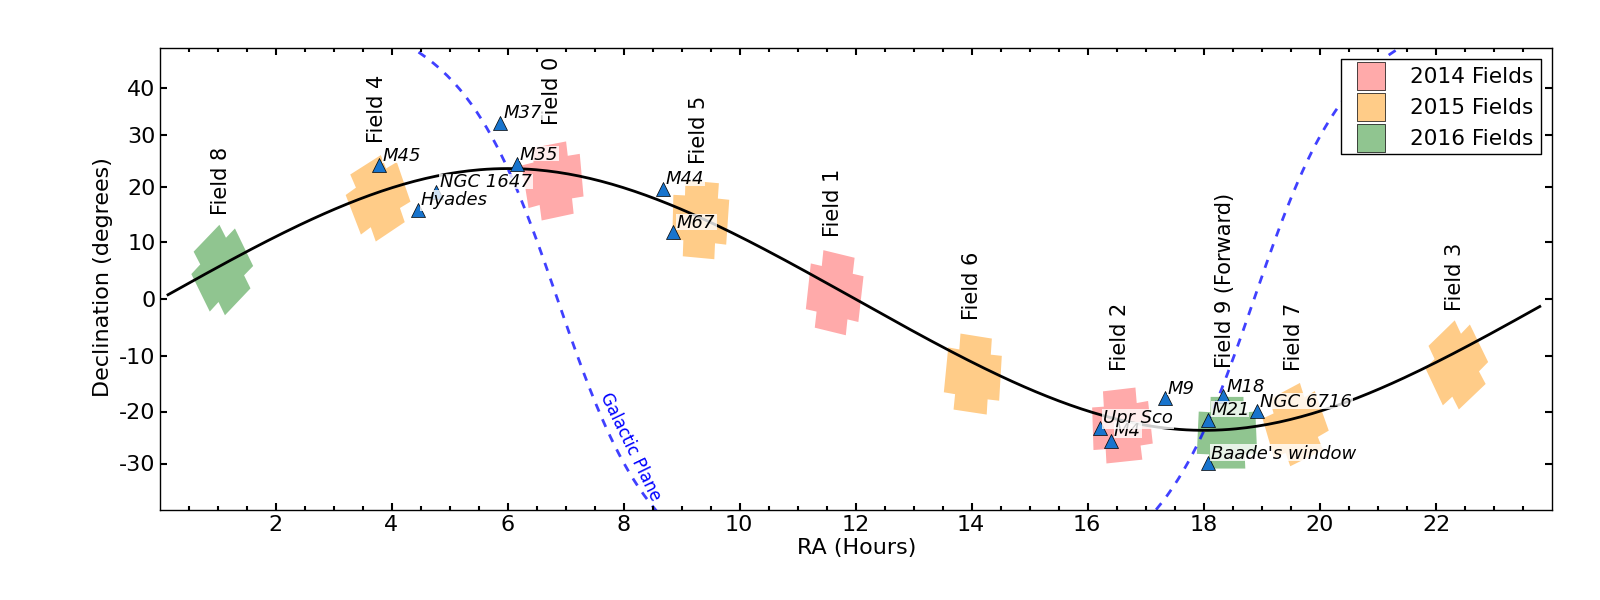
\includegraphics[width=\textwidth]{KeplerCampaignSky.png}\\
\begin{center}
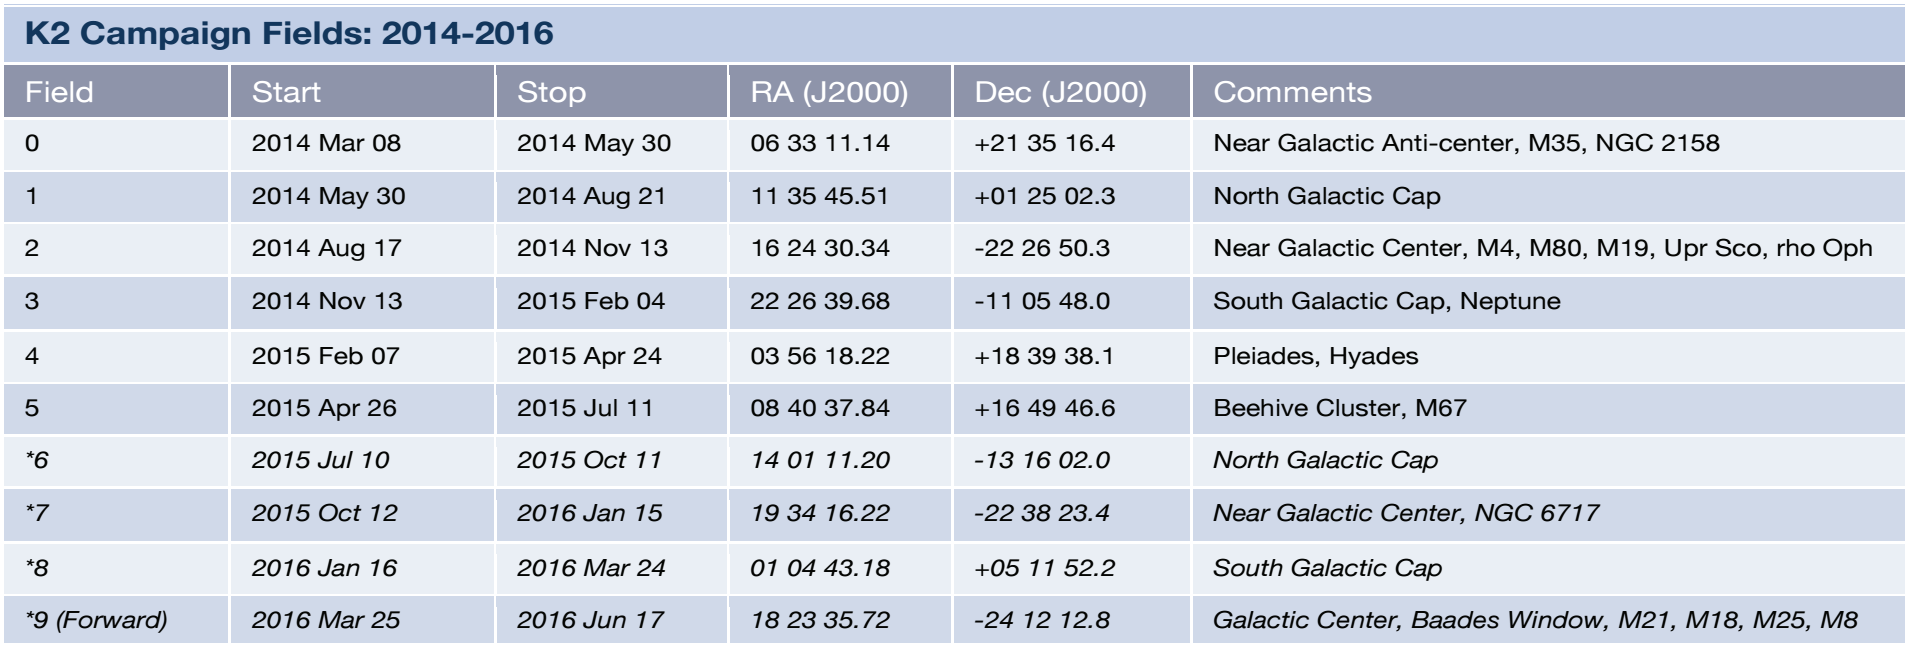
\includegraphics[width=0.8\textwidth]{K2table.png}\\
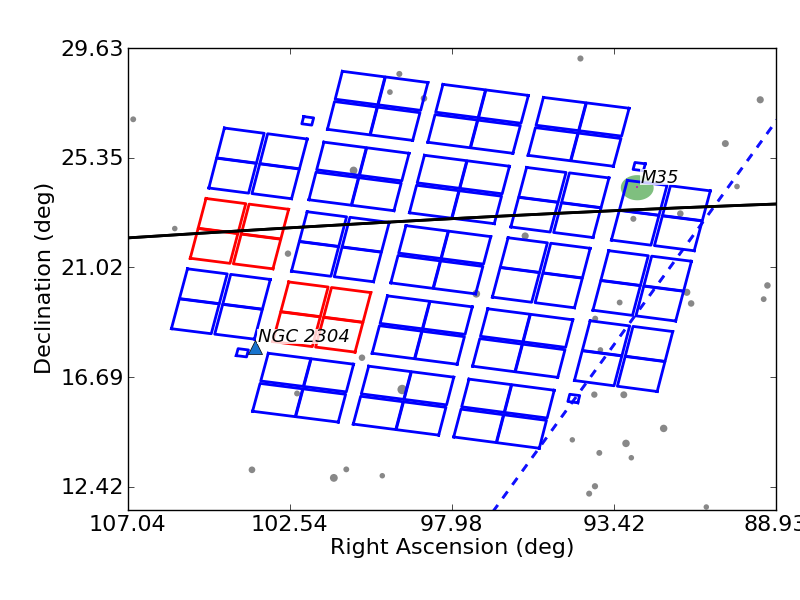
\includegraphics[width=0.6\textwidth]{Field0.png}\\
\end{center}

\subsection*{Joel Hartman Background}
Joel has been a very helpful resource throughout this project. He  works on HATNet and HatSouth transient surveys.
He searches for variable stars, including transiting planets orbiting bright stars. 
Joel created an open-source light curve analysis program called VARTOOLS, which includes methods for calculating variability and periodicity statistics of light curves. I've been encouraged to use this software, however, it is less visually intuitive than Waqas Bhatti's python-written software Astrobase. Both options are available.

\chapter*{User Accounts, Access, Data Locations}
G. Bakos contacted former postdoc Miguel de Val-Borro (now employed by NASA) to create an account for me on the relevant servers. I am now in the hatuser and hatpipebin groups. Bakos says we will discuss later whether I need an account on TRAC (e.g. hatreduc), but not for the time being.

\begin{minted}{bash}
    msoares@phs11.astro.princeton.edu
\end{minted}

The K2 pipeline is installed on phs3 and there is some raw data available under /nfs/phs3/ar1/ (91\% full at this time). As of 09/16/2015, Field 0 data were moved by Chelsea to phs11 for image subtraction. I now pretty much only use phs11.

\section*{Raw Data Location}
Chelsea downloaded K2 data from Campaigns 0, 1, and 2. I really only need to use Campaign 0 data at this point in time.
\begin{itemize}
\item \textbf{Campaign 0 -- data is under reduced on server phs11 (image subtraction necessary)}
\item Campaign 1 -- fully reduced light curve on server phs3 
\item Campaign 2 -- under reduced on server phs11 (image subtraction necessary)
\end{itemize}

Directories used by Chelsea:
\begin{itemize}
\item  phs3 $\rightarrow$ /nfs/phs3/ar1 (close to full)
\item phs11 $\rightarrow$ /nfs/phs11/ar0
\item \textcolor{blue}{The data I want are located on phs11 in the subdirectory\\ \textbf{/S/PROJ/hatuser/2015\_K2/K2\_0} (read only files)}
\end{itemize}

\subsection*{Data Reduction Location}
I will be reducing my data in a different location to help keep track of my personal project. This reduced data directory is: \textbf{/nfs/phs11/ar0/S/PROJ/msoares} with the K2.0 cluster data being stored in \\ \textbf{201509\_K20\_ISM\_OpenClusters}, a sub-directory therein. 
When making changes to the kernels to optimize the procedure, I am using directory: \\
\textbf{/nfs/phs11/ar0/S/PROJ/hatuser/2015\_K2/experiments}

\section*{Guidance from Chelsea}
\subsection*{Basics}
I had trouble getting the \textbf{fi} (shell scripts written by Joel) commands to work at all, but this was due to not having the tools in my pathway. Chelsea moved a file called \textbf{chelseaPYTHON27PATH} to my home directory. I can access these new tools by doing the following command:\\
\textbf{. chelseaPYTHON27PATH}\\ I have set up the alias \textbf{run} to do this quickly. \\ \\
Tab completing the prefix \textbf{fi} shows a host of tools, all shown in the image below.\\
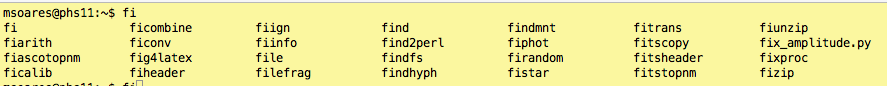
\includegraphics[width=\textwidth]{fitools.png}\\ \\
To get a sense of how to appropriately use the tool \textbf{fitrans}, I can use the \textbf{--long-help} command.\\
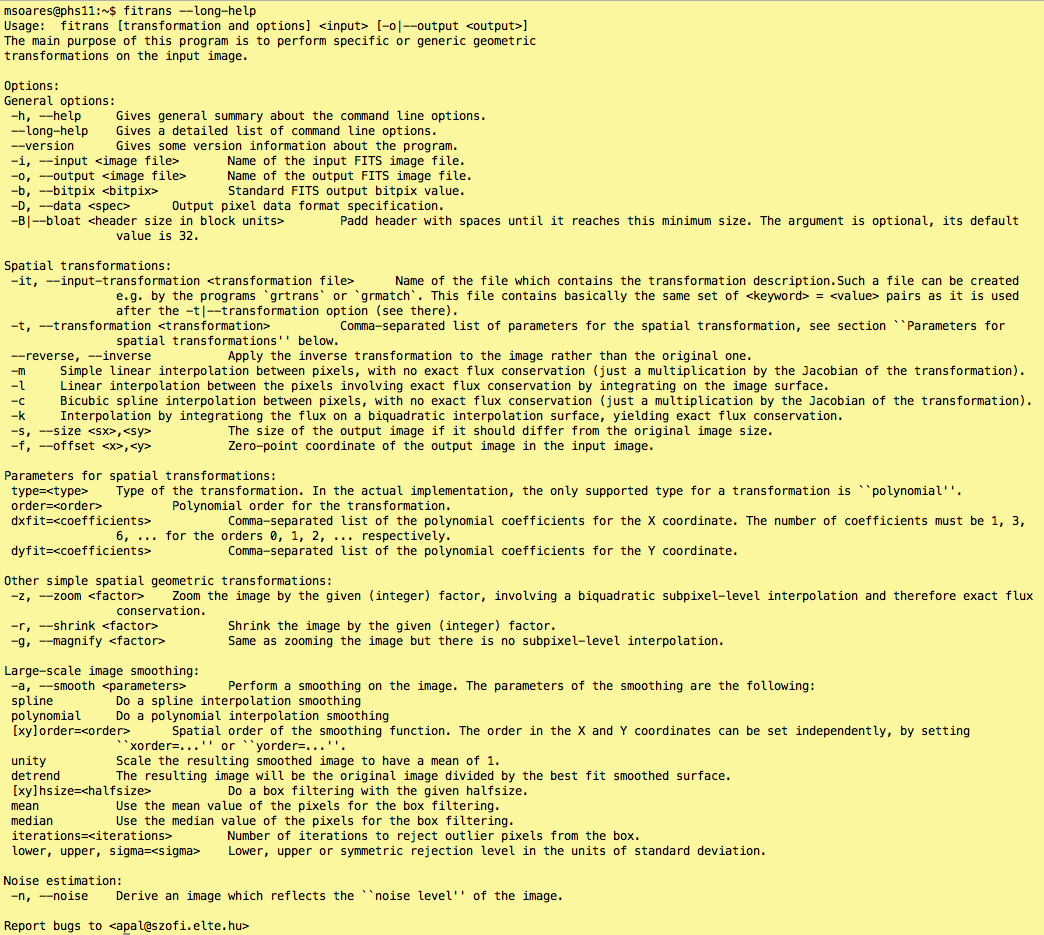
\includegraphics[width=0.8\textwidth]{help.png}\\

Chelsea explained that there are three major steps to the image subtraction process: 
\begin{enumerate}
\item \textit{relative astrometry -- image translation}
\item \textit{photometry reference -- creating a stacked frame}
\item \textit{final image subtraction -- subtracting to leave behind a variable field}
\end{enumerate}
The final image subtraction step requires a series of iterative steps to properly tune the kernel parameters. 

\subsection*{The K2 Field 0 Data Set}
Data files are located in phs11 in the directory \textbf{/S/PROJ/hatuser/2015\_K2/K2\_0}. However, a quick check at the start of the project revealed that the files were not located here. This is not a problem as the pointer to the files still works in my subdirectory \\ \textbf{/S/PROJ/msoares/201509\_K20\_ISM\_OpenClusters}.
\\ \\
There are two sub directories created by Chelsea: \textbf{Raw} and \textbf{Red}. The \textbf{Raw} folder contains the raw fits files downloaded directly from Kepler. These files contain relevant header information. This header information is sadly stripped away in the \textbf{Red} fits files. The \textbf{Red} folder contains files that have been stitched together into a single frame for a given time stamp (cadence) producing a larger field of view. These files are broken up into many directories, which indicate a particular \textbf{sky group number}. There are 84 sky group numbers in total.\\ \textcolor{blue}{My sky group number of interest (\textit{for both clusters}) is \textbf{x-81}.} \\ \\ Directory: \textbf{/S/PROJ/hatuser/2015\_K2/K2\_0/RED/Sgn-81}\\ \\ 
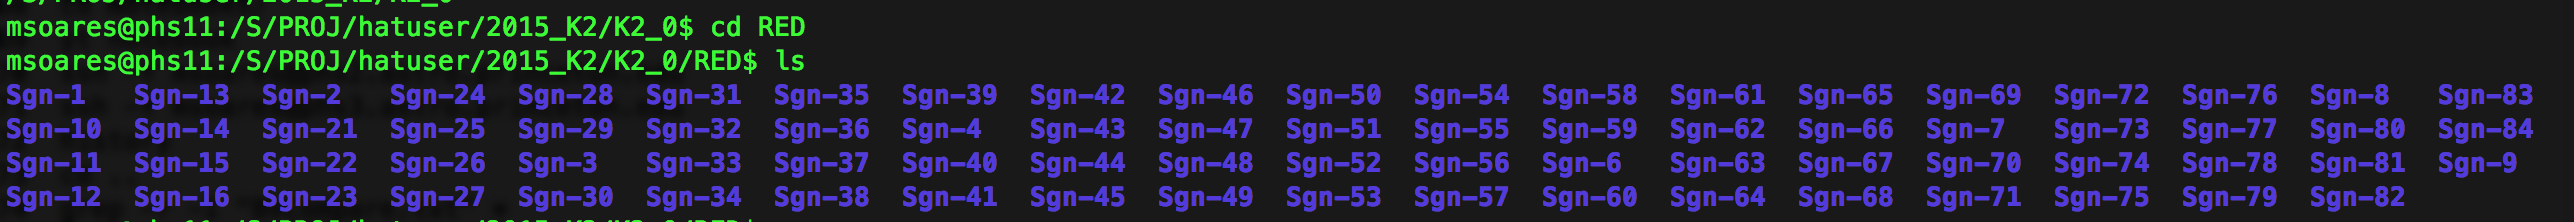
\includegraphics[width=\textwidth]{subdir.png}\\
I can go ahead and ignore the sky group number distinction as only the files for my particular sky group number are shown in the subdirectory: \\
\textbf{/S/PROJ/msoares/201509\_K20\_ISM\_OpenClusters/REDFITS}.\\ \\
Once inside Sgn-81, there are 4,846 files therein. 
Half of these files are \textbf{.fistar} files (explained shortly) and the other half are \textbf{.fits} files.\\
Here is a breakdown of the file naming scheme:
\begin{itemize}
\item FFI $\leftarrow$ ``full frame image''
\item -00- $\leftarrow$ K20
\item -81- $\leftarrow$ sky group number 81
\item 0001.fits $\leftarrow$ cadence number (time stamp) 
\end{itemize}
The cadence number sometimes skips values, so to create an animation I need to use \textbf{glob} and \textbf{sort} to handle these files rather than a simple iteration process.\\ 
I can look at the fits files using a simple ds9 command, for example:\\ 
\textbf{ds9 FFI-00-81-0110.fits $\&$}\\ This is also a great way to play with the scaling, inspect regions, etc. I will need to become better acquainted with ds9 to make this process less clunky. \\
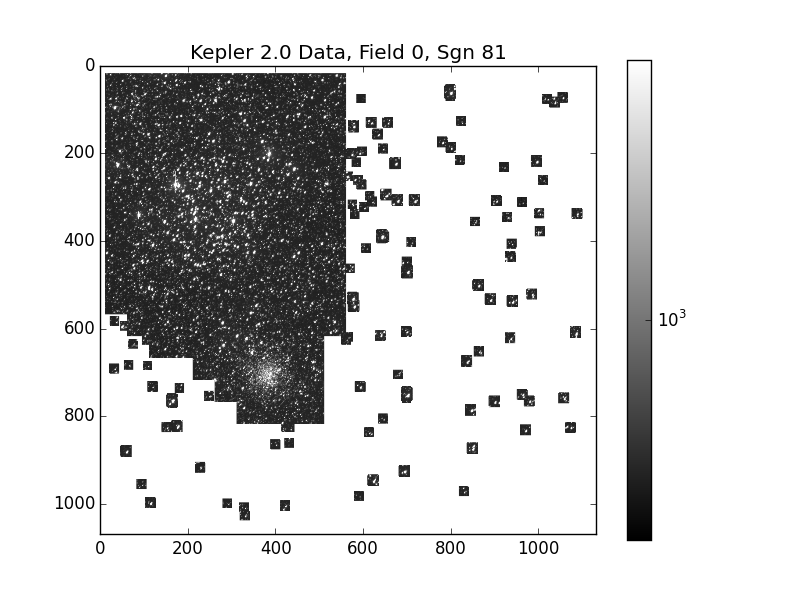
\includegraphics[width=\textwidth]{imagefile.png}\\
I've also created a Python script \textbf{2015\_0922\_MakeMovie.ipynb} that generates output .png images, which can then be strung together via Quicktime to make movies. This script will come in handy in the future when I want to sanity check that my rotated frames have been shifted appropriately. All Python notebook scripts are being kept in the following directory: \textbf{\/Users/msoares/Dropbox/K20/Notebooks}.
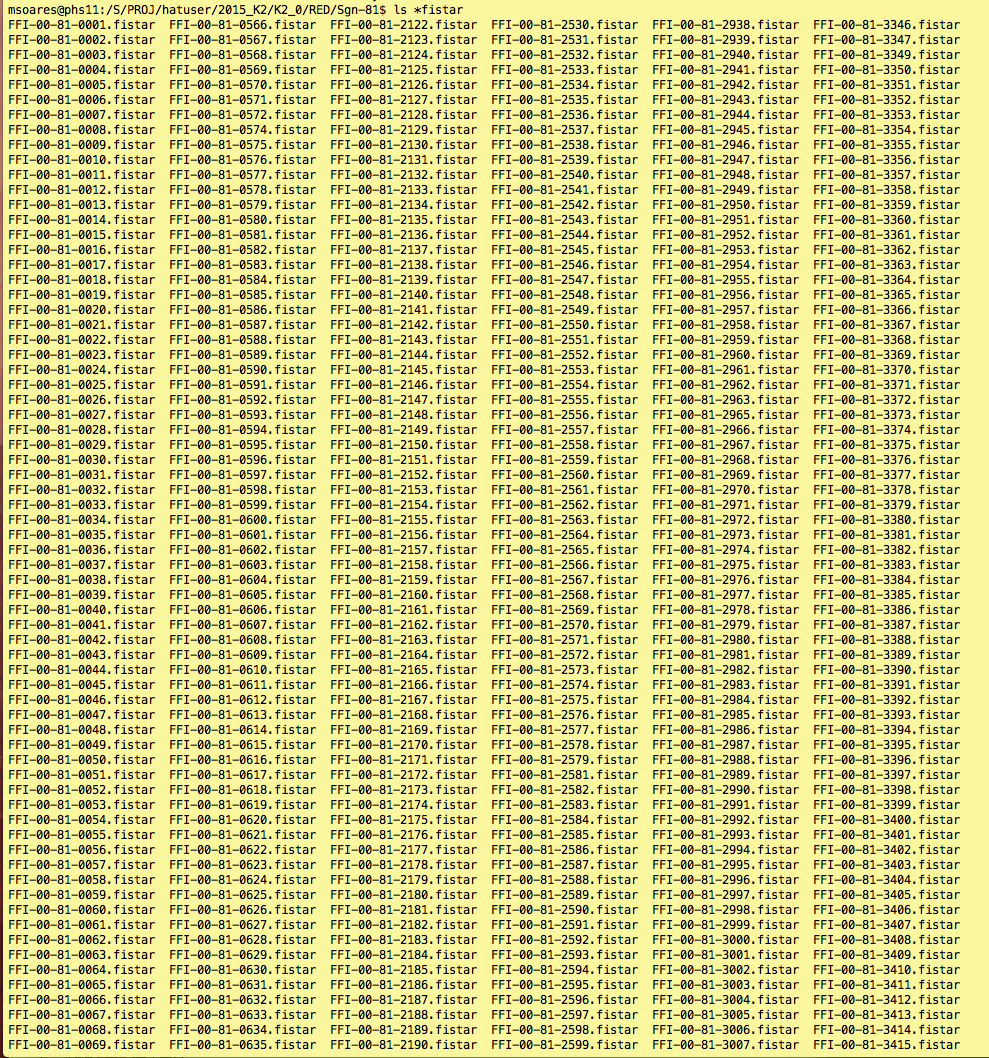
\includegraphics[width=0.6\textwidth]{files2.png}\\
I also have a python script called \textbf{MakeMovie.py} in the \textbf{/home/msoares/chelseasrc/ims} subdirectory.

\subsubsection*{Fistar Files}
The \textbf{.fistar} file is really just a simple text file with the sources extracted. 
These have already been created by Chelsea for my region of interest. To create these files, Chelsea used the \textbf{fistar} command (hence the name):\\ \\
\textbf{fistar /S/PROJ/hatuser/2015\_K2/K2\_0/RED/Sgn-81/FFI-00-81-2121.fits -o \\ 
/S/PROJ/hatuser/2015\_K2/K2\_0/RED/Sgn-81/FFI-00-81-2121.fistar -s flux --comment --model elliptic --flux-threshold 500 --algorithm uplink --iterations symmetric=2,general=1 --format id,x,y,bg,amp,flux,s/n --only-candidates} \\ \\ 
This is shown in the text file image below. The command sets a flux threshold. The uncertainties of the fistar source extractor is about 0.07 pixels. \\ 
I ended up having to remake the stitched fits frames, as Chelsea used an early data release, so this is a step I ended up implementing.\\

\begin{center}
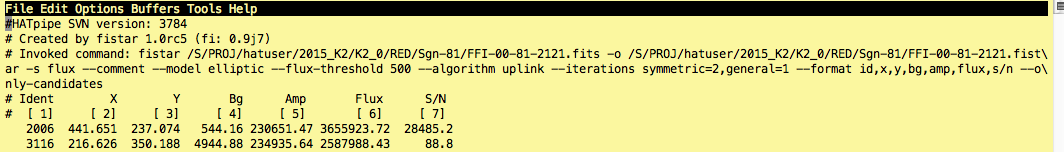
\includegraphics[width=\textwidth]{fistarfile.png}
\end{center}
\subsection*{Creating the Inlist File}
These \textbf{.fistar} files are then read into Chelsea's script \textbf{run\_grmatch.py}, located in my directory \\  \textbf{/home/msoares/chelseasrc/ims}. To quickly go to this directory, use the alias \textbf{xu}. 
This directory contains lots of simple Python scripts written by Chelsea to perform various \textbf{fi} functions.
Each of these fistar files is called through an inlist file, specified in the \textbf{run\_grmatch.py} script. 
\textit{This list of fistar files is the first thing I need to create.} \\ 
The way to do this is to select a subset of files that have an RA or DEC that does not change very much with time and put the pathways to these files in a simple text file, which I've named \textbf{inputlist.ls}. 
In order to find out which files belong on this list, plot the RA or DEC versus time (time being the variable \textbf{cadence} in our case) and determine the subset of files that show up along a horizontal line (with little scatter) where statistically the most data points occur. 
There is initially a good deal of scatter, as shown in the plot below.
\begin{center}
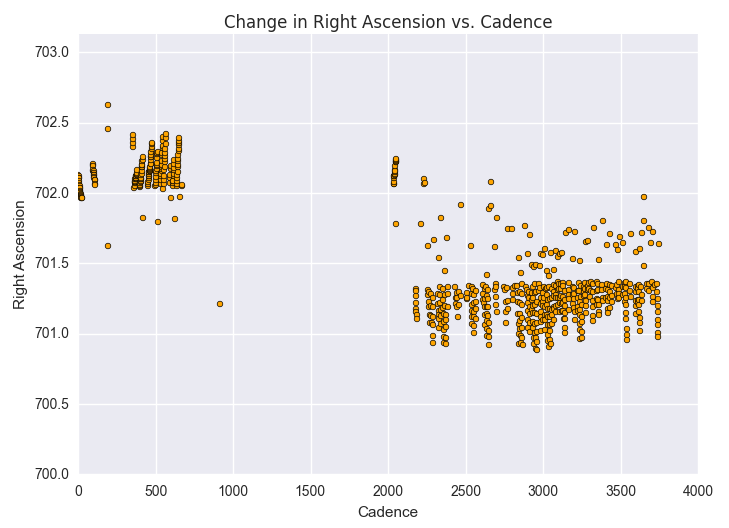
\includegraphics[width=0.7\textwidth]{scatter.png}
\end{center}
You can arbitrarily be as strict as you like with the scatter threshold. Tuning this to get $\sim$40 files is suggested.\\
\begin{center}
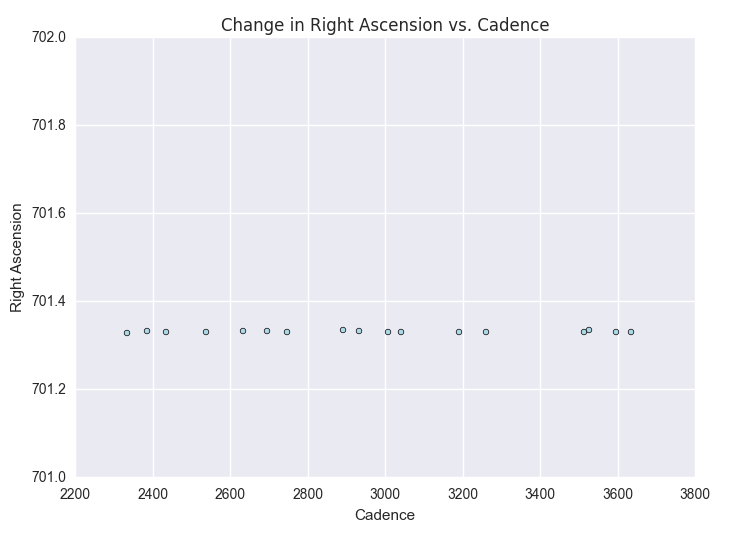
\includegraphics[width=0.6\textwidth]{line.png}
\end{center}
I have created a script which does this automatically, using a simple \textbf{awk} command and outputs the filenames for the input list.\\ \textbf{/Users/msoares/Dropbox/K20/Notebooks/2015\_0925\_PLOTXYShift.ipynb}  \\ 
\textbf{/Users/msoares/Dropbox/K20/Notebooks/2016\_0107\_SelectingStackedImages.ipynb}

\subsection*{Script I: \textbf{run\_grmatch.py}}
I have modified Chelsea's original \textbf{run\_grmatch.py} to use my proper directories and save the generated \textbf{.itrans} files to a directory where I have write privileges. This new script is cleverly named \textbf{melinda\_run\_grmatch.py}. Initially, all the \textbf{.itrans} files are piped to:\\
\textbf{/nfs/phs11/ar0/S/PROJ/msoares/201509\_K20\_ISM\_OpenClusters/IMSUB}. Although, all this piping gets changed so that they currently reside in \textbf{/nfs/phs11/ar0/S/PROJ/hatuser/2015\_K2/experiments/C0} \\
Also necessary to run the script is the \textbf{reference file}, which is just a selected fistar file. \textit{\textbf{melinda\_run\_grmatch.py} sets the coordinate reference frame of the final stacked image}. The selection of this file is not arbitrary, however, and I should set it to the sharpest file. I do this by checking the FWHM and PSF.
Once generated, I can open the outputted \textbf{.itrans} files. \textit{These are simple text files listing the translations necessary to put each of the inlist files into the new master coordinate reference frame.} 
Shown below is the output of one such file.\\
\begin{center}
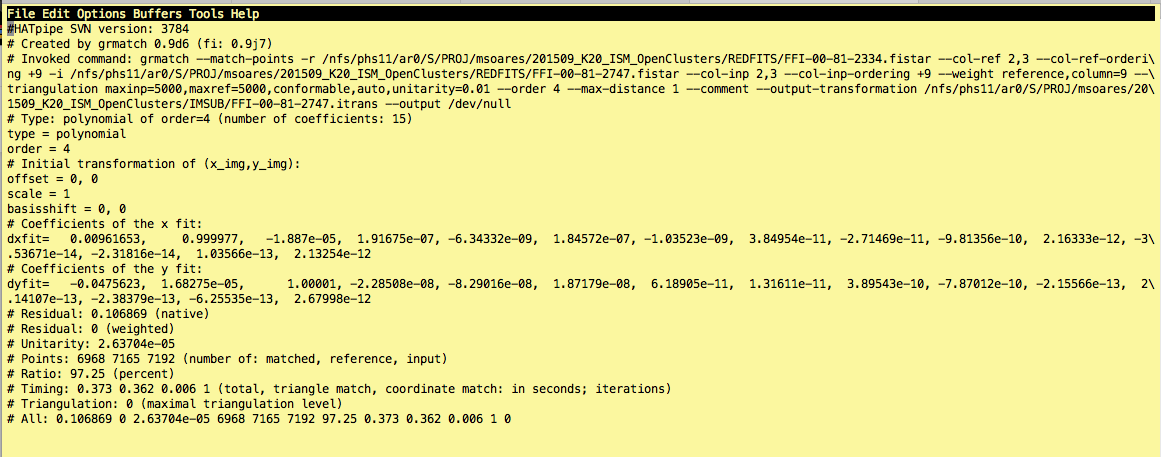
\includegraphics[width=\textwidth]{itrans.png}
\end{center}
Make sure that the output is sane by checking that both the \textbf{Residual} and \textbf{Unitarity} values are low. 
I need to also ensure that the \textbf{Ratio} is above 70\%. \\ \textit{Next, I actually perform the transformations and get all the files in the same master coordinate reference frame.} 

\subsection*{Script II: \textbf{trans\_ref.py}}
I also have modified Chelsea's original script \textbf{trans\_ref.py} and renamed this new python script \textbf{melinda\_trans\_ref.py}. This script contains 109 lines of code. 
The script requires an inlist file, which I have named \textbf{inputlist2.ls} (this was called fits.ls when I first performed the procedure). This is a list of the pathways to our subset selection of raw fits images. I generate this with the same iPython notebook I use to determine the subset of files I am going to use \\ \textbf{/Users/msoares/Dropbox/K20/Notebooks/2015\_0925\_PLOTXYShift.ipynb}\\

Essentially, the file is really just using the \textbf{directtrans\_multi} function. 
Chelsea had the script set up so that the output files would be placed in the same directory as the RAW data, however I do not have write privileges in these directories. Instead I am piping everything to the directory: \textbf{/nfs/phs11/ar0/S/PROJ/msoares/201509\_K20\_ISM\_OpenClusters/IMSUB}. 
This is the same directory that contains the \textbf{.itrans} files. These new outputted files are fits file with the ending \textbf{xtrns.fits}. We have since changed the piping, so that itrans and xtrns files go into their own \textbf{IMS} subdirectory folders with the same name. The \textbf{IMS} directory is housed within: \textbf{/nfs/phs11/ar0/S/PROJ/hatuser/2015\_K2/experiments/C0}\\
Pipelines are controlled in the script \textbf{setting.py}.
The command being invoked is: \\ \\
\textbf{fitrans /nfs/phs11/ar0/S/PROJ/msoares/201509\_K20\_ISM\_OpenClusters/REDFITS/FFI-00-81-3261.fits -k --input-transformation /nfs/phs11/ar0/S/PROJ/msoares/201509\_K20\_ISM \\ \_OpenClusters/IMSUB/FFI-00-81-3261.itrans --reverse -o /nfs/phs11/ar0/S/PROJ/msoares/ \\
201509\_K20\_ISM\_OpenClusters/IMSUB/FFI-00-81-3261-xtrns.fits}.\\ \\ 
These new output fits files have been shifted to our master coordinate reference frame and may be stacked. It is important to make sure that they look as though they have been shifted appropriately. I do this by creating .png image files from the .fits files and then stringing them together to a quick movie to ensure that stars do not shift as the movie loops. The script to automate this is \textbf{2015\_0922\_MakeMovie\_ShiftedFrames.ipynb}, also my script 
\textbf{/home/msoares/chelseasrc/ims/MakeMovie.py} works for this as well. 
I string the films together via Quicktime. The shifted files looks great, so now I can move on to actually stacking the images.

\subsubsection*{Masking Files}
If my files are already masked then I can skip this section. 
I need to check my xtrns and my photref files to see if they are masked. 
It's probably worthwhile to mask them before the transformation procedure.
Do not forget to check the photref file!
Files need to be masked before performing image subtraction. 
The command is of the following form:\\ 
\textbf{fiign -i afitsfile -n -o newfitsfile \\
fiign -i photreffile -n -o newphotreffile}
More accurately, the command I used was: \\
\textbf{fiign -i FFI-00-81-3595-xtrns.fits -n -o FFI-00-81-3595-xtrns\_fiign.fits}\\
\textbf{fiign -i photoref-00-81.fits -n -o photoref-00-81\_fiign.fits}\\
Running the fiign command, as shown below, creates a masked file, which can be viewed in ds9. Using the command: \\
\textbf{fiign -i infile -a -m -999 -o outfile}\\
generates an outfile with all masked pixels set to the value `999', as shown in the image below. 
\begin{center}
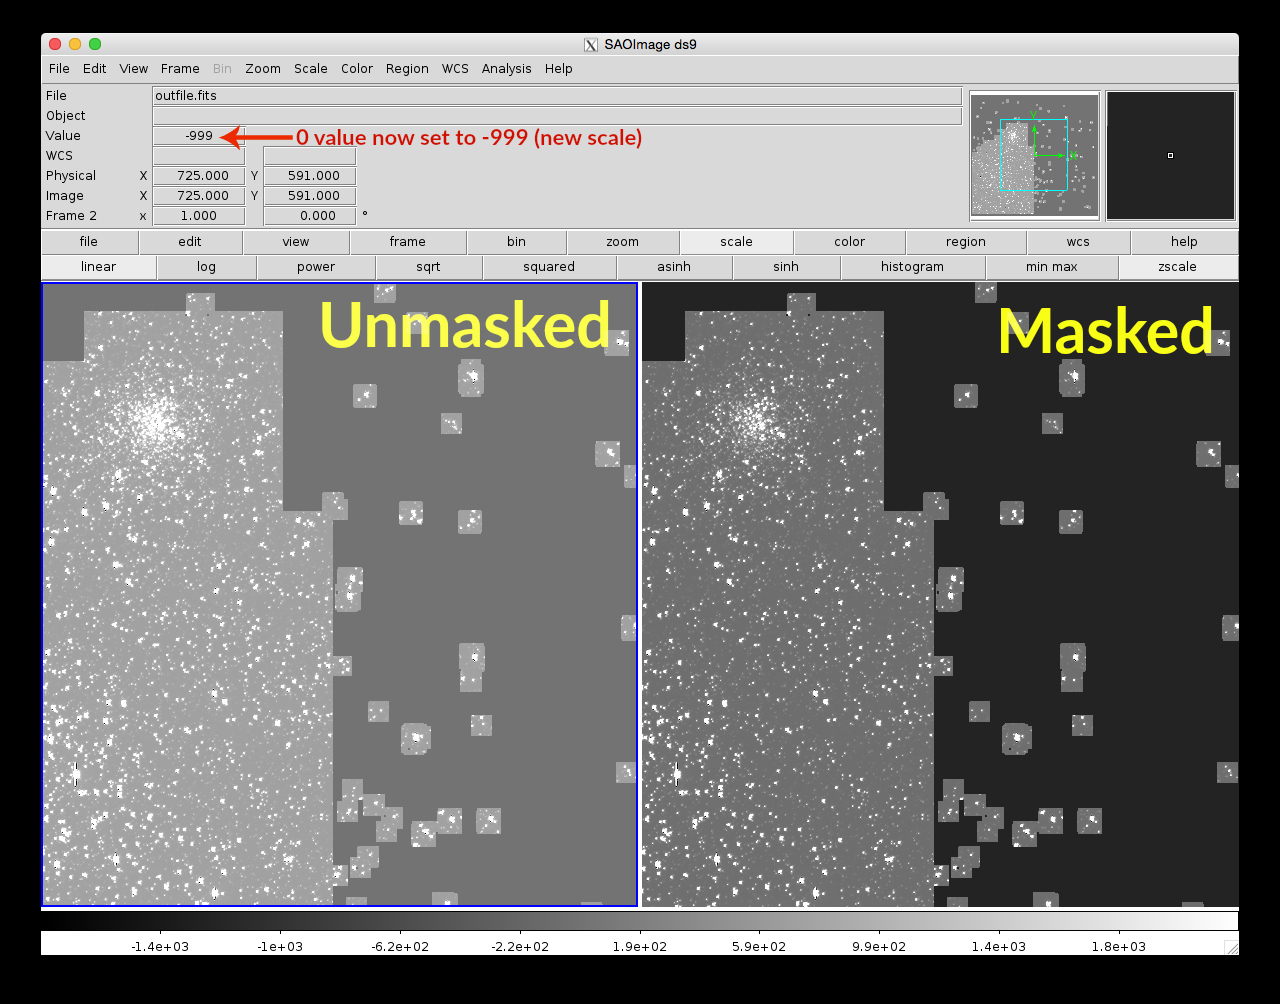
\includegraphics[width=0.9\textwidth]{masked.jpg}
\end{center}

\textcolor{red}{\textit{Joel has mentioned that it is important to ensure that the masking tool is working accurately. To do so I need to overplot the regions to ensure that they do not overlap with bad or empty parts of the image. If this is the case, it will throw the fit off. Write a script to check this!}}

\subsection*{Stacking Image Files to Generate the Photo Reference Frame}
Essentially in this step I just take the median/mean flux values of all frames in the PHOTREF directory (the subset hand picked to ensure not too much RA and DEC variance) and make a new frame. It will turn out that we get better results if we stack the entirety of the data set and not just a subset. Stacking is a very easy process with just one simple \textbf{ficombine} command where I take the \textbf{-xtrns.fits} files, specify the median as the chosen mode of operation, and write an output pathway, here chosen to be again in my IMSUB sub-directory. I have chosen the naming prefix \textbf{photoref-00-81} to indicate the field number and sgn number. I experiment with taking both the median and mean flux values and find that the mean works better. 

The used command is given here:\\
\textbf{ficombine /nfs/phs11/ar0/S/PROJ/msoares/201509\_K20\_ISM\_OpenClusters/IMSUB/*-xtrns.fits --mode median -o /nfs/phs11/ar0/S/PROJ/msoares/201509\_K20\_ISM\_OpenClusters/IMSUB \\ /photoref-00-81.fits}\\
The latest version of this command (01/2016) is given here: \\
\textbf{ficombine /nfs/phs11/ar0/S/PROJ/hatuser/2015\_K2/experiments/40\_stacked/IMS/xtrns/*xtrns.fits --mode median -o /nfs/phs11/ar0/S/PROJ/hatuser/2015\_K2/experiments/40\_stacked/PHOTREF/ \\ PhotRef.fits}

I then open up this newly created photref fits image in ds9 and try to get a sense of whether or not these results are sane. Chelsea has warned me that sometimes a wonky image will have strange black streaks. Luckily, I have a sane looking photref fits file, as shown below.
\begin{center}
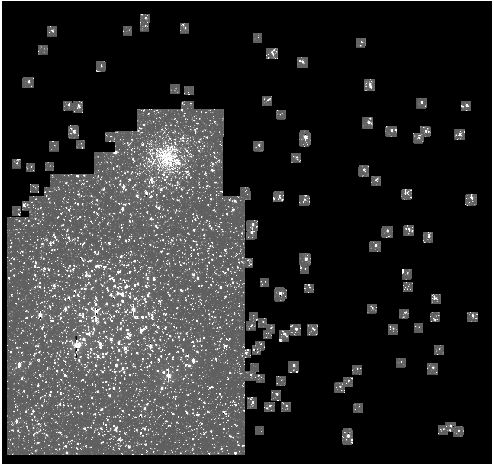
\includegraphics[width=0.5\textwidth]{median.png}
\end{center}
Also, to get a sense of the proper scale, open up a second fits image in ds9 and match the two scales. 

\subsubsection*{Using \textbf{ficonv} + \textbf{ficombine}}
A better way to stack the images is to use \textbf{ficonv}. This method, however, builds upon the prior, as it will use the outputted photoref file described in the previous section. 
To start the ficonv+ficombine process, I need to generate something called a \textbf{region file}. The region file gives \textbf{ficonv} an idea of the position of bright stars on the frame to have a good initial start.
The way to go about doing this is to use the script regslct.py, which I have edited and renamed as \textbf{melinda\_regslct.py}.
This script has a single function in it and takes in a \textbf{fistar} file. Joel recommends using the highest focused image, however with Kepler it is unlikely that the focus will change much. To determine the sharpest focused image, check the median value for the \textbf{s} parameter in the \textbf{.fistar} files, which is the inverse variance of the star.
\textcolor{red}{Why not just go with the smallest value of the FWHM or the largest \textbf{s} value instead?}\\ \\ 
\textcolor{red}{\textit{After reviewing the script with me, Chelsea recommended that I raise the saturation value to 300,000, which seemed high to me. Joel says that tuning the saturation value was of significant importance.}}\\ \\ 
Running \textbf{melinda\_regslct.py} outputs three columns of text, which are then copied and pasted into a \textbf{.reg} file. This, however, has now been automated.
Files were formally named to reflect choice of cadence (\textbf{2334.reg}), however this too has been updated to name all region files as the arbitrary \textbf{PhotRef.reg} and place them in their proper PHOTREF directory. 
Double check the following values in the script: \textbf{colflux},  \textbf{xsize}, and \textbf{ysize}.
The latter two variables can be determined by checking the fits header. See how to do this with \texttt{150922\_Exploring\_Fits\_Data.ipynb}.
\begin{center}
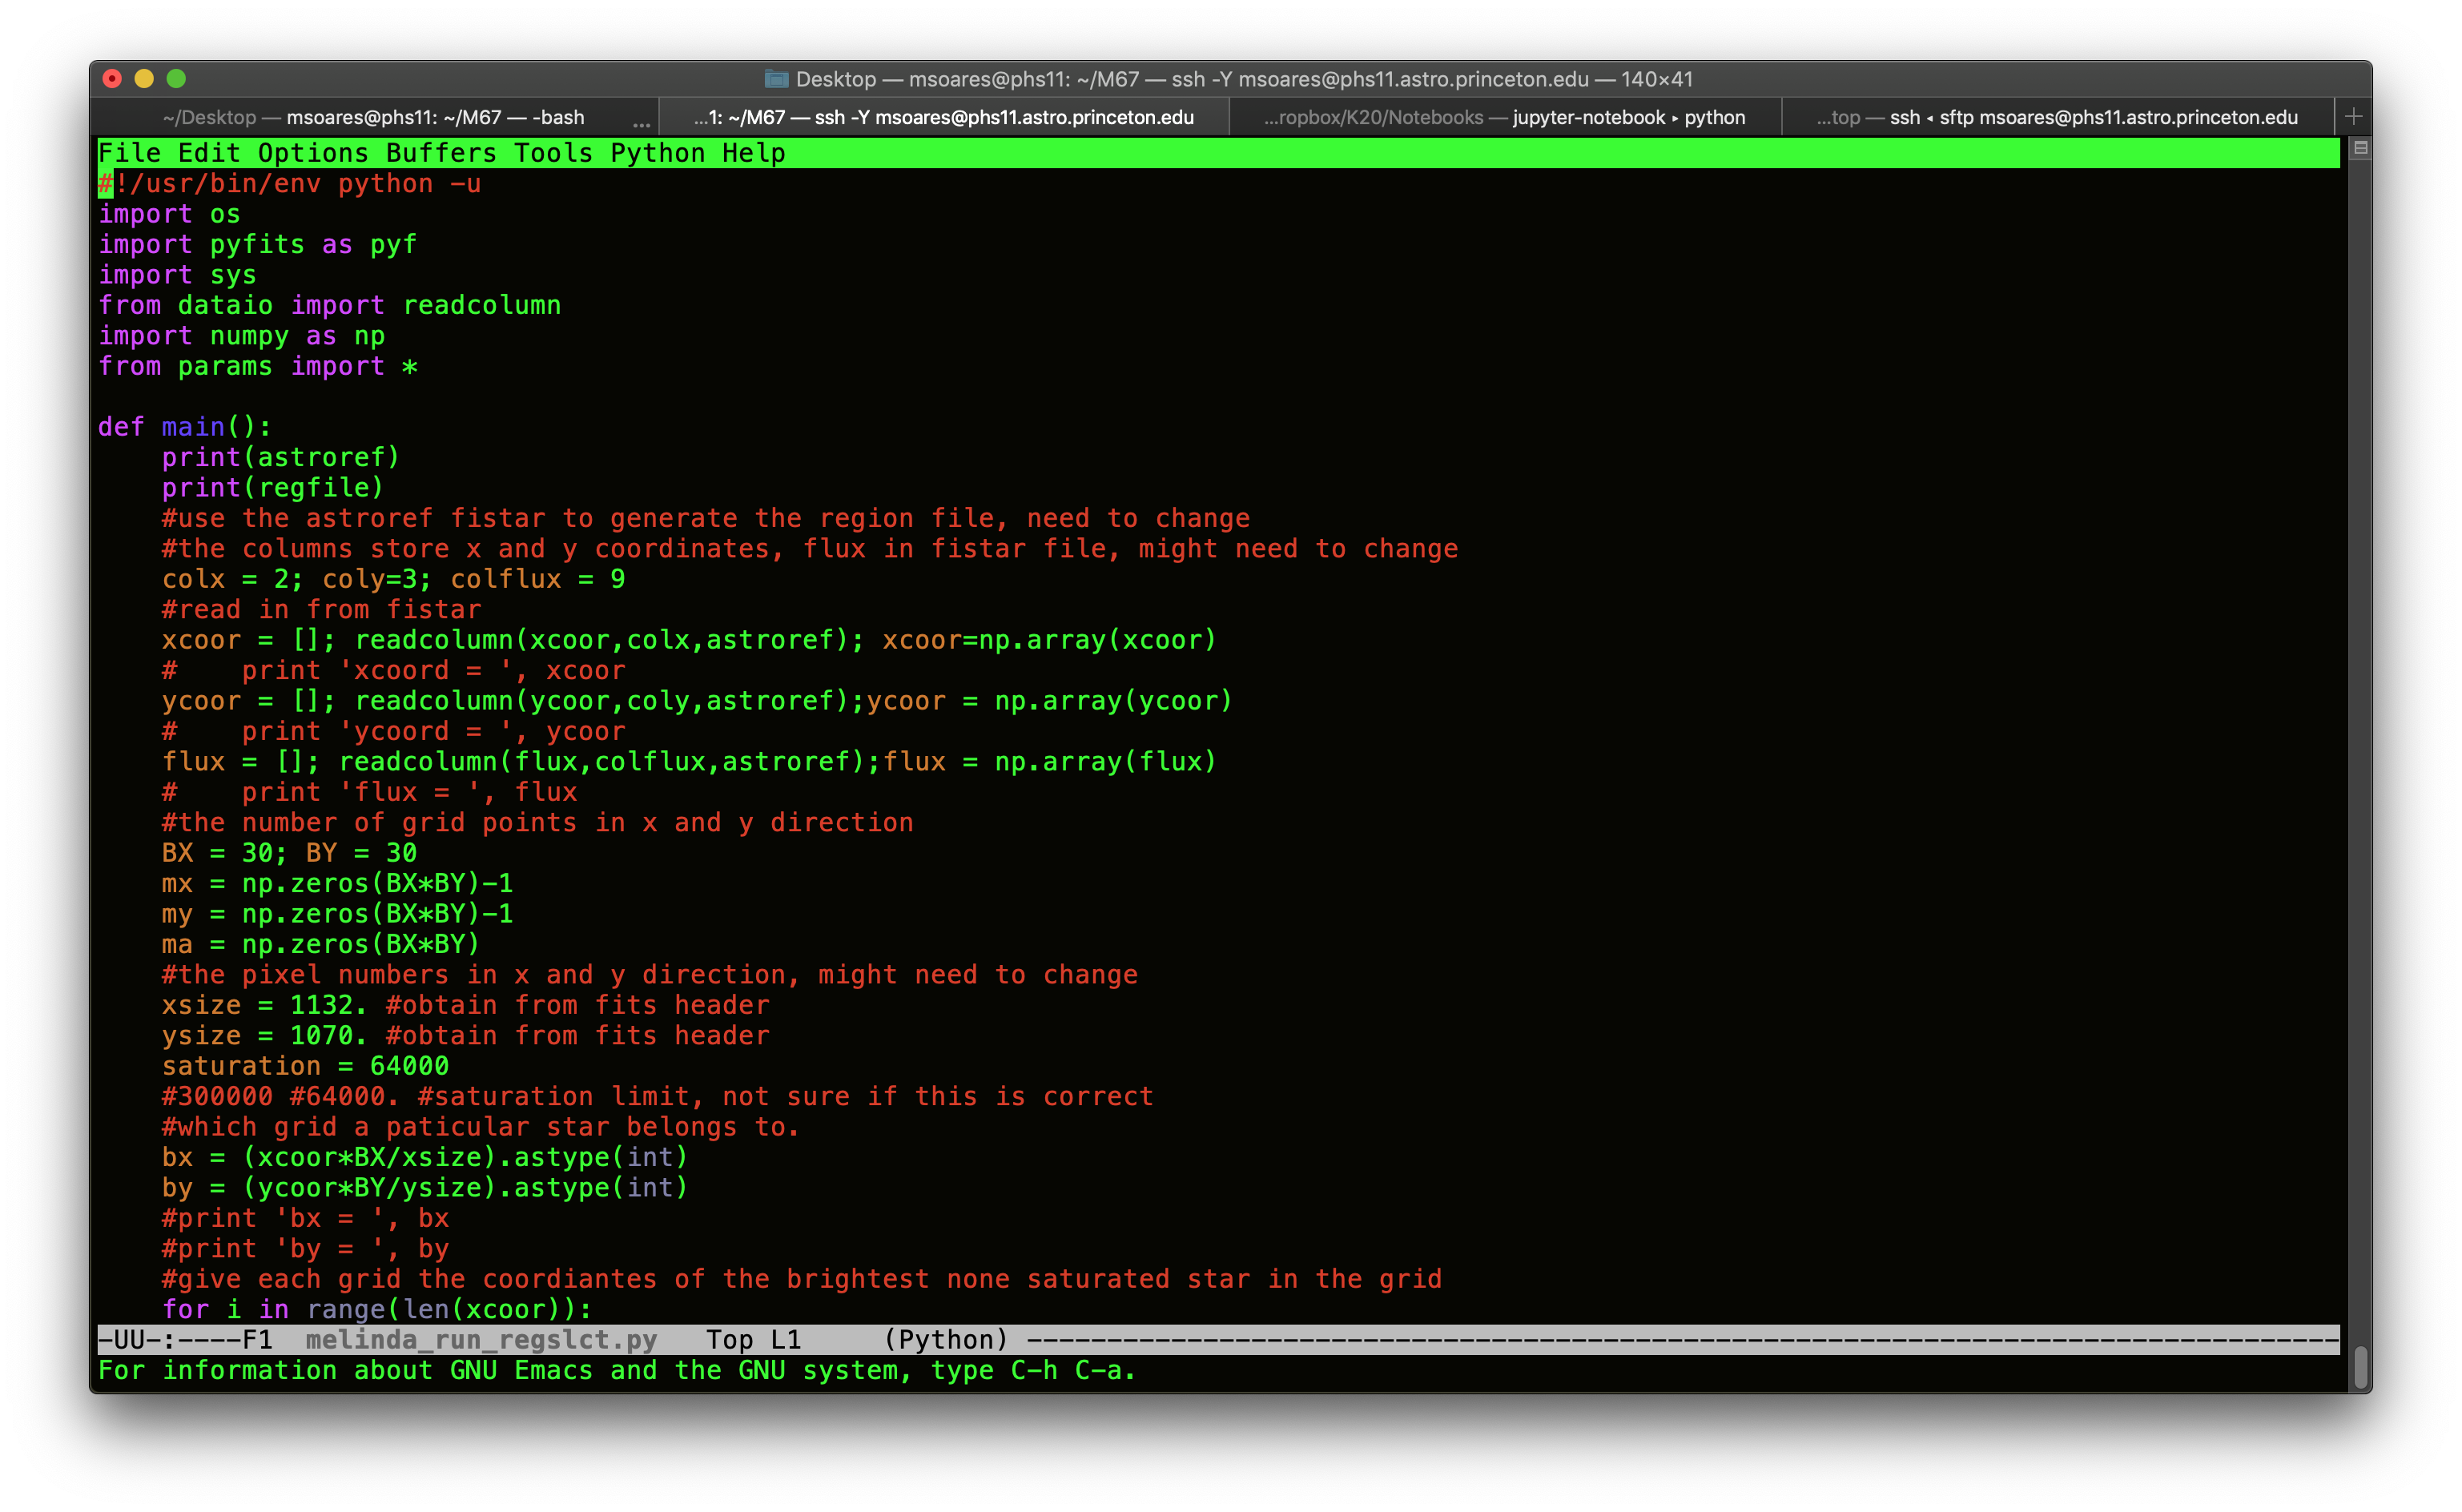
\includegraphics[width=0.8\textwidth]{regslct.png}
\end{center}
\begin{center}
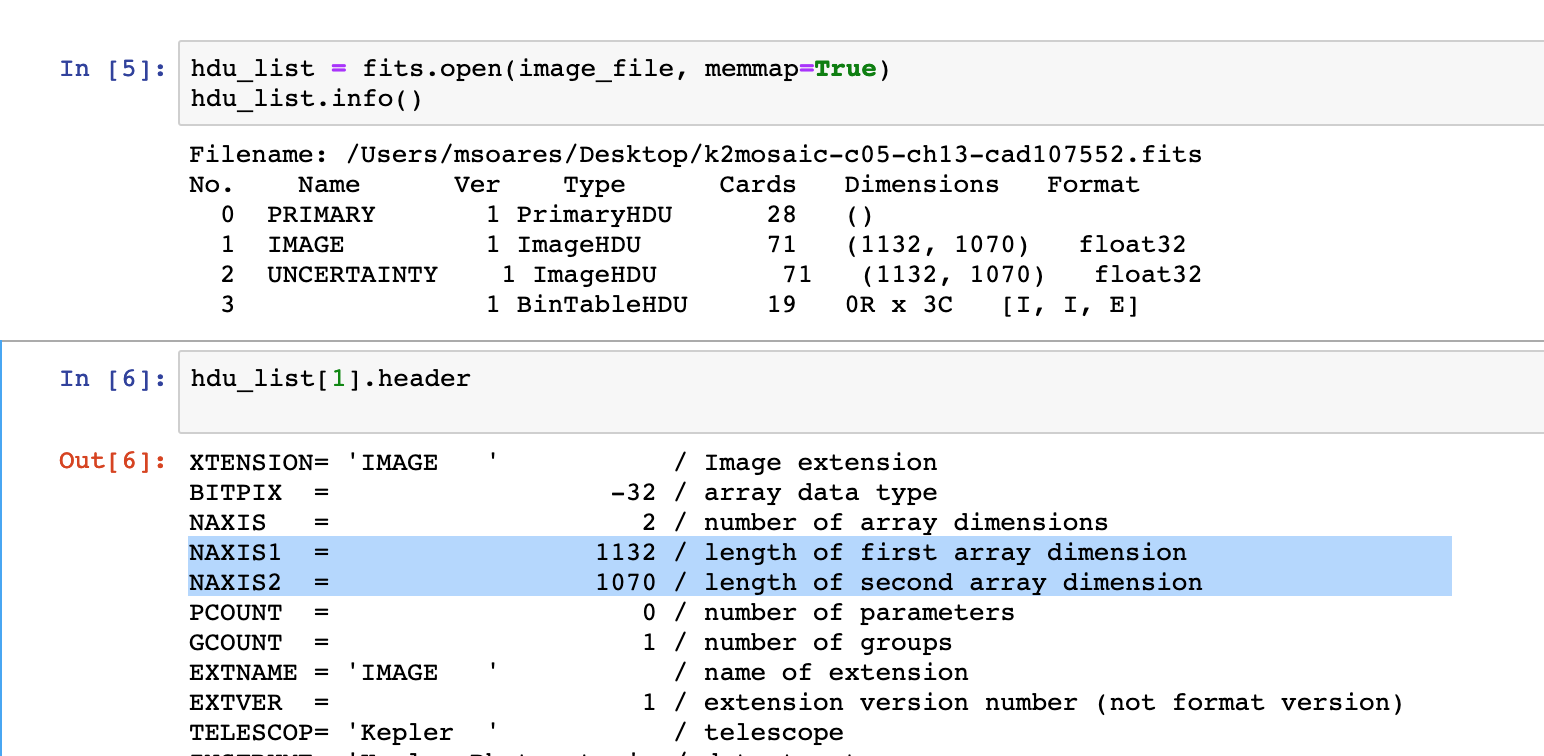
\includegraphics[width=0.8\textwidth]{header.png}
\end{center}

\subsubsection*{Script: run\_ficonv.py}
Next, I run Chelsea's script \textbf{run\_ficonv.py}, which I have renamed \textbf{melinda\_run\_ficonv.py} to reflect changes made. This is file containing 155 lines, which takes a \textbf{.itrans}, \textbf{xtrns}, and a \textbf{region} file to run. I also use the stacked photref frame as the file that the other fits files are compared to and then subtracted off. This is called the \textbf{reffile} in the script. I double checked this with Chelsea and this is indeed the right way to go about it. \\
Running \textbf{melinda\_run\_ficonv.py} results in the output of \textbf{.kernel} and \textbf{-sub.fits} files. \\ 
The script has compared the psf of all the frames and convolved the files to have the least sharpest psf. 
The next step is to simply combine the images.

%%%LEFT OFF HERE FOR NOTEBOOK EDITING%%%%

\subsection*{Subtraction}
Chelsea recommended that I incorporate an output file and do the subtraction from the command line. A simple change of the \textbf{os} option to the \textbf{oc} option allows me to output the file that we will subtract. \\
\textbf{fiarith "'/nfs/phs11/ar0/S/PROJ/msoares/201509\_K20\_ISM\_OpenClusters/IMSUB/FFI-00-81-3595\_fiign-xtrns.fits'-'/nfs/phs11/ar0/S/PROJ/msoares/201509\_K20\_ISM\_OpenClusters/IMSUB/FFI-00-81-3595\_fiign-subtract.fits'" -o /nfs/phs11/ar0/S/PROJ/msoares/201509\_K20\_ISM\_OpenClusters/IMSUB/FFI-00-81-3595\_fiign\_diff.fits}\\
\textcolor{red}{\textit{Of course, I will need to automate this process.}}\\
Below is an example of a first test run of a subtracted image, as compared to the raw data.
\begin{center}
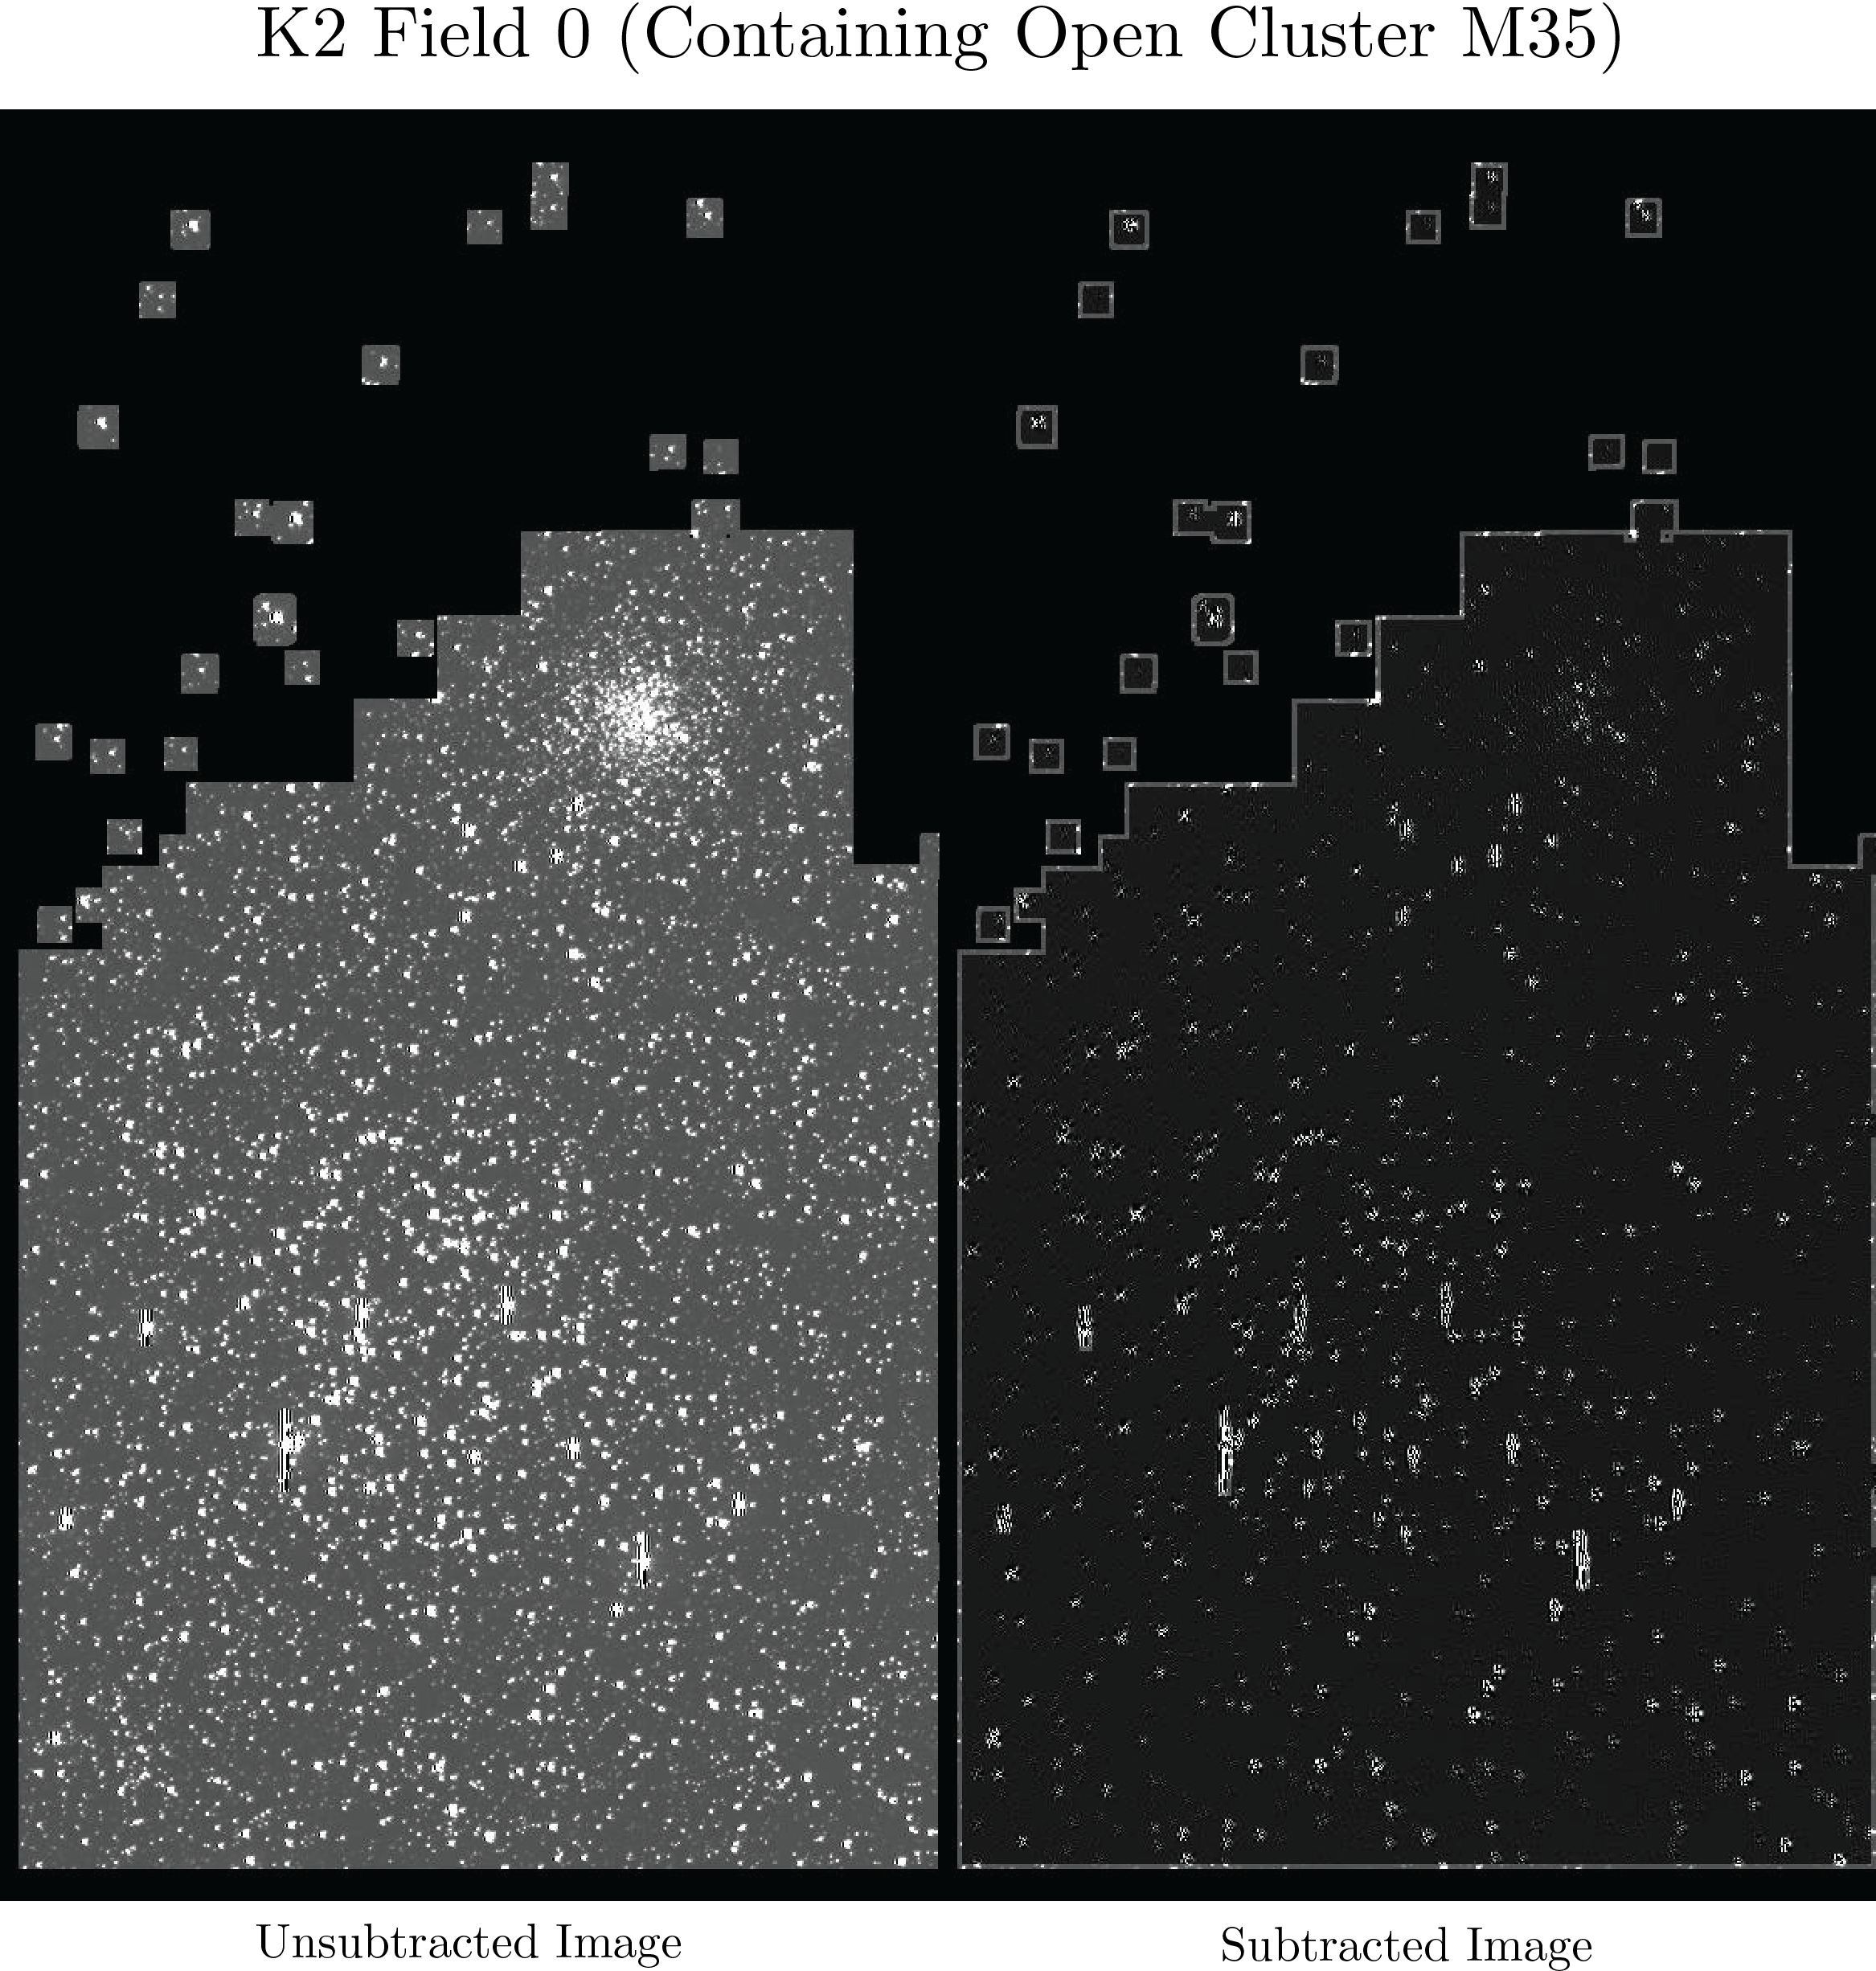
\includegraphics[width=0.8\textwidth]{Figure1Proposal.png}
\end{center}

The next task is to fine tune the parameters of the \textbf{melinda\_run\_ficonv.py} script. These parameters include \textbf{b}, \textbf{i}, \textbf{d} in the script. Joel claims I should start with nice low numbers, perhaps even 0! 

\subsection*{High Resolution Photref -- photometry with subtracted image}
Chelsea sent me an email with a helpful, in-depth description of the this step.\\  

Doing normal aperture photometry on the master image (i.e. the photometry reference), requires: 
\begin{enumerate}
\item \textbf{fiphot} - program used for aperture photometry
\item list of x,y coordinates for the stars we want to do photometry on 
\item fits image (photoref, with regions properly masked)
\item list of aperture to do the photometry on **start with a big list, making plots, and then choose the good few ones. 
\item method to convert magnitude to flux, I had a guess for Kepler, which is not too bad 
\end{enumerate}

All stars I query will have temporary HAT identifier numbers. 
After I release the light curve it will be linked to UCAC numbers.

The script that does the high-resolution photometry procedure is the shell script, \textbf{cmrawphot.sh}, however Chelsea recently wrote up a Python script for this bit.
The Python script is in the \textbf{chelseasrc} directory and is called \textbf{run\_iphot.py}. I renamed a version of this as \textbf{melinda\_run\_iphot.py}. I filled in the inputs referring to my past instruction and the \textbf{cmrawphot.sh} scripts and tested it on a few frames.\\ In order to work, I had to address a pickling error with a \textbf{copy\_reg module} workaround. It is now working fine, but it does take some time to run -- \textit{approximately 30 minutes or so}.

\subsubsection*{Getting list of x and y coordinates} 
\hl{Skip this for now!}\\ \\
\textit{How to get a list of x,y coordinates of stars?}\\
Chelsea already has this list compiled, so I can skip this bit. Here is the relevant background: \\
The file Chelsea made is called \textbf{photref.cat}
This is done by getting the astrometry solution on the photo ref/astro ref. 
Let's assume I have a file provided by Chelsea called \textbf{photref.trans}. 
This transfile is similar to the \textbf{itrans} file I used before, 
except it provides the polynomial transformation between 
$x_{i}$, $\eta$ $\rightarrow$ x,y (itrans provides the transformation between x,y $\rightarrow$ x,y). 
Usually this match has a worse result compared to the x,y$\rightarrow$x,y match.\\ 
Of course, for each of the stars, I only know about the RA and DEC.
$x_{i}$ and $\eta$ are obtained by calculating the distance of this star to a 
field center RA0 and DEC0, using a tangent transformation. 
So, there are two steps of transformation:
\begin{itemize}
\item RA and DEC $\rightarrow$  $x_{i}$ and $\eta$ (requires RA0 and DEC0) 
\item RA0 and DEC0 are read from the second to last line of the \textbf{transfile}.
\end{itemize}
\textcolor{red}{\textit{Review this above at a later time.}}\\ \\ 
The transformation itself is performed by calling: \\
\textbf{grtrans --input catfile --col-radec 2,3 --wcs 'tan,ra=rac,dec=dec,degrees' --col-out 5,6 --output outfile}\\ \\
$x_{i}$ and $\eta$ $\rightarrow$ RA and DEC (requires the transformation file)\\
\textbf{grtrans --input outfile (from above) --col-xy 5,6 -col-out 5,6 --input-transformation transfile --output starlistfile}

\subsubsection*{Photometry on Subtracted Frames}
This entire procedure is self-contained in the \textbf{melinda\_run\_iphot.py} script and therefore this bit can be ignored. 
This portion of the procedure actually performs photometry on the subtracted frames and uses the raw photometry from the master frame to infer the actual flux/magnitude of each stars on the non-subtracted frames. \\
This is done by calling the shell script, \textbf{IMG-3-PHOT\_M35.sh}.

Required to know:
\begin{itemize}
\item path for various files
\item raw photometry file
\item aperture list we used for raw photometry file
\item subtracted fits file
\end{itemize}
This script also requires the \textbf{itrans} file, the \textbf{JD} (or cadence or serial number) for each frame so later on I can generate light curves much easier. \\ \\
First the script calls the \textbf{fiphot} program in the subtracted frame photometry mode,then it transforms one sets of x,y coordinates back into the original frame coordinate using the \textbf{.itrans file}, and finally it prints out other relevant information that the light curve requires. \\ \\
 \textcolor{red}{\textit{Prints this ``relevant information'' in what format? Is this just the newly generated \textbf{.iphot} frames and the \textbf{photref\_M35.cmraw.phot} file?}}

\subsection*{Collecting the Light Curves}
Light curve collection is performed by calling the program \textbf{grcollect}. \\
See Chelsea's bash script \textbf{lc\_gen.sh}. 
The script takes a input list, which we have named \textbf{iphot.ls}. This input list contains frame names without an extension or pathway.
I can open the input list iphot.ls as an example. 
I then tell the script where the lightcurve goes by changing the value of LC.
The script reads in all the iphot (photometry) files at one time, and match the measurement for the same star from different frames, and output light curve files (.rlc).
Lightcurves are being generated and saved to the pathway \textbf{/nfs/phs11/ar0/S/PROJ/msoares/201509\_K20\_ISM\_OpenClusters/IMSUB/LC/}.
You run the script with the command \textbf{./lc\_gen.sh}, however I have renamed this to \textbf{melinda\_lc\_gen.sh}\\
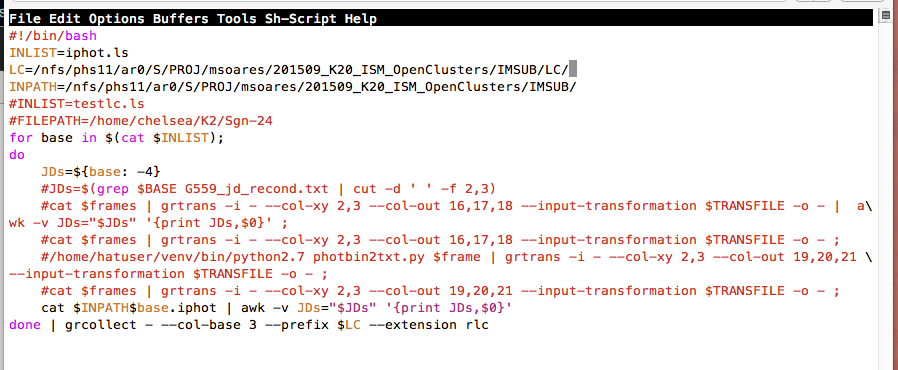
\includegraphics[width=0.9\textwidth]{lcgen.png}\\
\\ \\ 

\section*{Comparing Light Curves}
The next step is to compare my newly generated lightcurves to those published by other sources (Nardiello et al. 2014). 
I should start with things brighter than \textbf{13th V-mag} and with \textbf{variation amplitude $>$ 1\%}.\\ \textcolor{red}{\textit{How do I check variation amplitude? Is this just as easy as it sounds?}}\\
This would give a solid first impression for the quality of our light curve. 
I will then gradually go down on mag and precision during the fine tuning process. 

I need the HAT ID number in order to compare light curves, To get this, I need the RA and DEC (in degrees) of the star, which is conveniently given in the catalog table of the Nardiello paper.
The command to run to determine the HAT ID for a given RA and DEC is: \\ 
\textbf{2massread -r ra -d dec -s 0.005 --cat /S/CAT/2MASS/2MASS\_JH\_AP/data/}.\\
This command is querying a star within 0.0005 degrees of the given RA and DEC. This really is the limit on how finely resolved we should make the query program. If multiple stars are within this field, I will need to look at the J and H magnitudes of the star to distinguish it from neighbors. 
I wrote the script \textbf{FindHatID.py}, which finds a HATID for a requested RA and DEC value. 
Output looks like the image below: \\
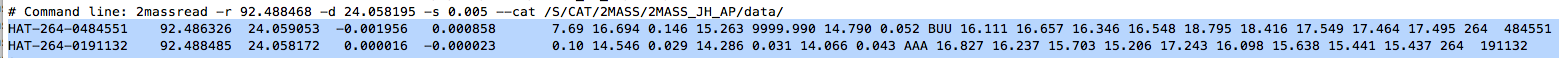
\includegraphics[width=\textwidth]{HATID.png}\\
The 7th column is the J-2MASS magnitude and the 9th column is the H-2MASS magnitude, which are both given in the catalog table in Nardiello et al. 2014. In this instance, we want HATID number \textbf{HAT-264-0191132}. This ID number is the title of the \textbf{.rlc} file of interest.\\
The larger Nardiello et al. catalog is given here:\\
\url{http://vizier.cfa.harvard.edu/viz-bin/VizieR-3?-source=J/MNRAS/447/3536/variable}\\ \\ 
I will be comparing the light curves of 10 selected objects. These stellar objects, their coordinates, their magnitudes, and the corresponding HAT ID numbers are given in the table below.


\begin{table}[]
\centering
\label{my-label}
\begin{tabular}{|c|c|c|c|c|c|c|c|}
\hline
\textbf{Star} & \textbf{RA} & \textbf{DEC} & \textbf{Type} & \textbf{$V_{\rm 2MASS}$} & \textbf{$J_{\rm 2MASS}$} & \textbf{$H_{\rm 2MASS}$} & \textbf{HAT ID} \\ \hline
%\textbf{Star} & \textbf{RA} & \textbf{DEC (+)} & \textbf{Type} & \textbf{V\_2MASS} & \textbf{J\_2MASS} & \textbf{H\_2MASS} & \textbf{HAT ID} \\ \hline
514           & 92.113065   & 24.328803        & EB            & 10.072            & 9.919             & 9.889             & HAT-264-0002367 \\ \hline
509           & 92.314359   & 24.258219        & Rot           & 10.175            & 9.918             & 9.957             & HAT-264-0002364 \\ \hline
506           & 92.439300   & 24.214583        & Rot           & 10.390            & 10.082            & 10.099            & HAT-264-0002883 \\ \hline
516           & 92.248379   & 24.366616        & Rot           & 10.685            & 10.256            & 10.260            & HAT-264-0264752 \\ \hline
512           & 92.199523   & 24.295566        & Rot           & 10.709            & 10.318            & 10.317            & HAT-264-0003539 \\ \hline
497           & 92.225659   & 24.369275        & Rot           & 10.874            & 10.493            & 10.460            & HAT-264-0004259 \\ \hline
517           & 92.45543    & 24.401628        & EB            & 12.569            & 11.527            & 11.460            & HAT-264-0016758 \\ \hline
508           & 92.128748   & 24.253384       & EB   		   & 12.744            & 11.648             & 11.399             & HAT-264-0016779 \\ \hline
513           & 92.409717   & 24.298180        & EB            & 12.924             & 11.262              & 10.961             & HAT-264-0012457 \\ \hline
515           & 91.971587   & 24.353585       & EB             & 13.132 & 12.150	           & 11.969              & HAT-264-0023455 \\ \hline

\end{tabular}
\caption{Comparison Selection for Light Curves  -Taken from Nardiello et al. 2014}
\label{Nard}
\end{table}

\section*{Generate the Light Curve}
Example walk-through:\\
I now have a file of interest, which in this case is file \textbf{HAT-264-0191132.rlc}. This is just a text file with lots of ``null'' values therein. 
I have a cadence column (column 1), and lots of magnitude columns. 
Next, \textit{for now},  I go on to download all \textbf{.rlc} plots, so I can use the interactive iPython notebook format to generate scripts. 
I'm currently using the notebook \textbf{2015\_1015\_PlotLightCurve.ipynb} to generate light curves for now. 
For now, I am ignoring optimization of the aperture selection for now. This will be the final step after I have finely tuned all other parameters.
\textit{Behold}, I can now plot magnitude vs. time, where $t \rm = 2456727.0219333335+cadence \times \frac{0.5}{24}- 2456000$ 
I am generating light curves in an interactive format using plotly. You can see my interactive plotly gallery at:\\
\url{https://plot.ly/~msoares/}.

\section*{First Light Curve Batch Results: \hl{\textbf{b}/2, \textbf{i}/3, and \textbf{d}=3/3}}
I generated light curves for the ten Nardiello sources listed in Table \ref{Nard}. These ten were selected because they were bright in J-magnitude. I preferentially selected eclipsing binaries when possible and ignored long period variables, where variability would be unlikely to be seen given our observation window. Unfortunately, this initial attempt was not successful. The oscillations shown in the light curves were caused by the variations due to drift and were not real photometric variations. 
The immediate next step was to \textcolor{red}{\textit{create a few sets of light curves varying the image subtraction parameters, and using a photometry master frame with each of the reference frames "ficonv"ed first.}}\\
Chelsea recommends the following parameter variation format:
\begin{itemize}
\item -k part of the ficonv command... changing the number after b/, i/ and d=;\\
where b/ controls the order of the polynomials fit to the background, i/ controls the order of polynomials we fit to the flux term of the kernel, and d=x/y, x is the size of the half size of the discrete kernel, y is the polynomial order. For all the numbers, Chelsea wouldn't go higher than 4.
She suspects x should be small, right now d=3/3, maybe I should try x=1 and 2 first. 
\end{itemize}
As recommended by Joel, I computed the standard deviation of each light curve and generated a scatter plot of average magnitude vs standard deviation for each aperture size. Joel claims that these plots are often informative diagnostics. 
This was generated using the code \textbf{StndVMag.py}. A snapshot of the script is shown below with the first containing HATSOUTH points overplotted for reference. 
\begin{center}
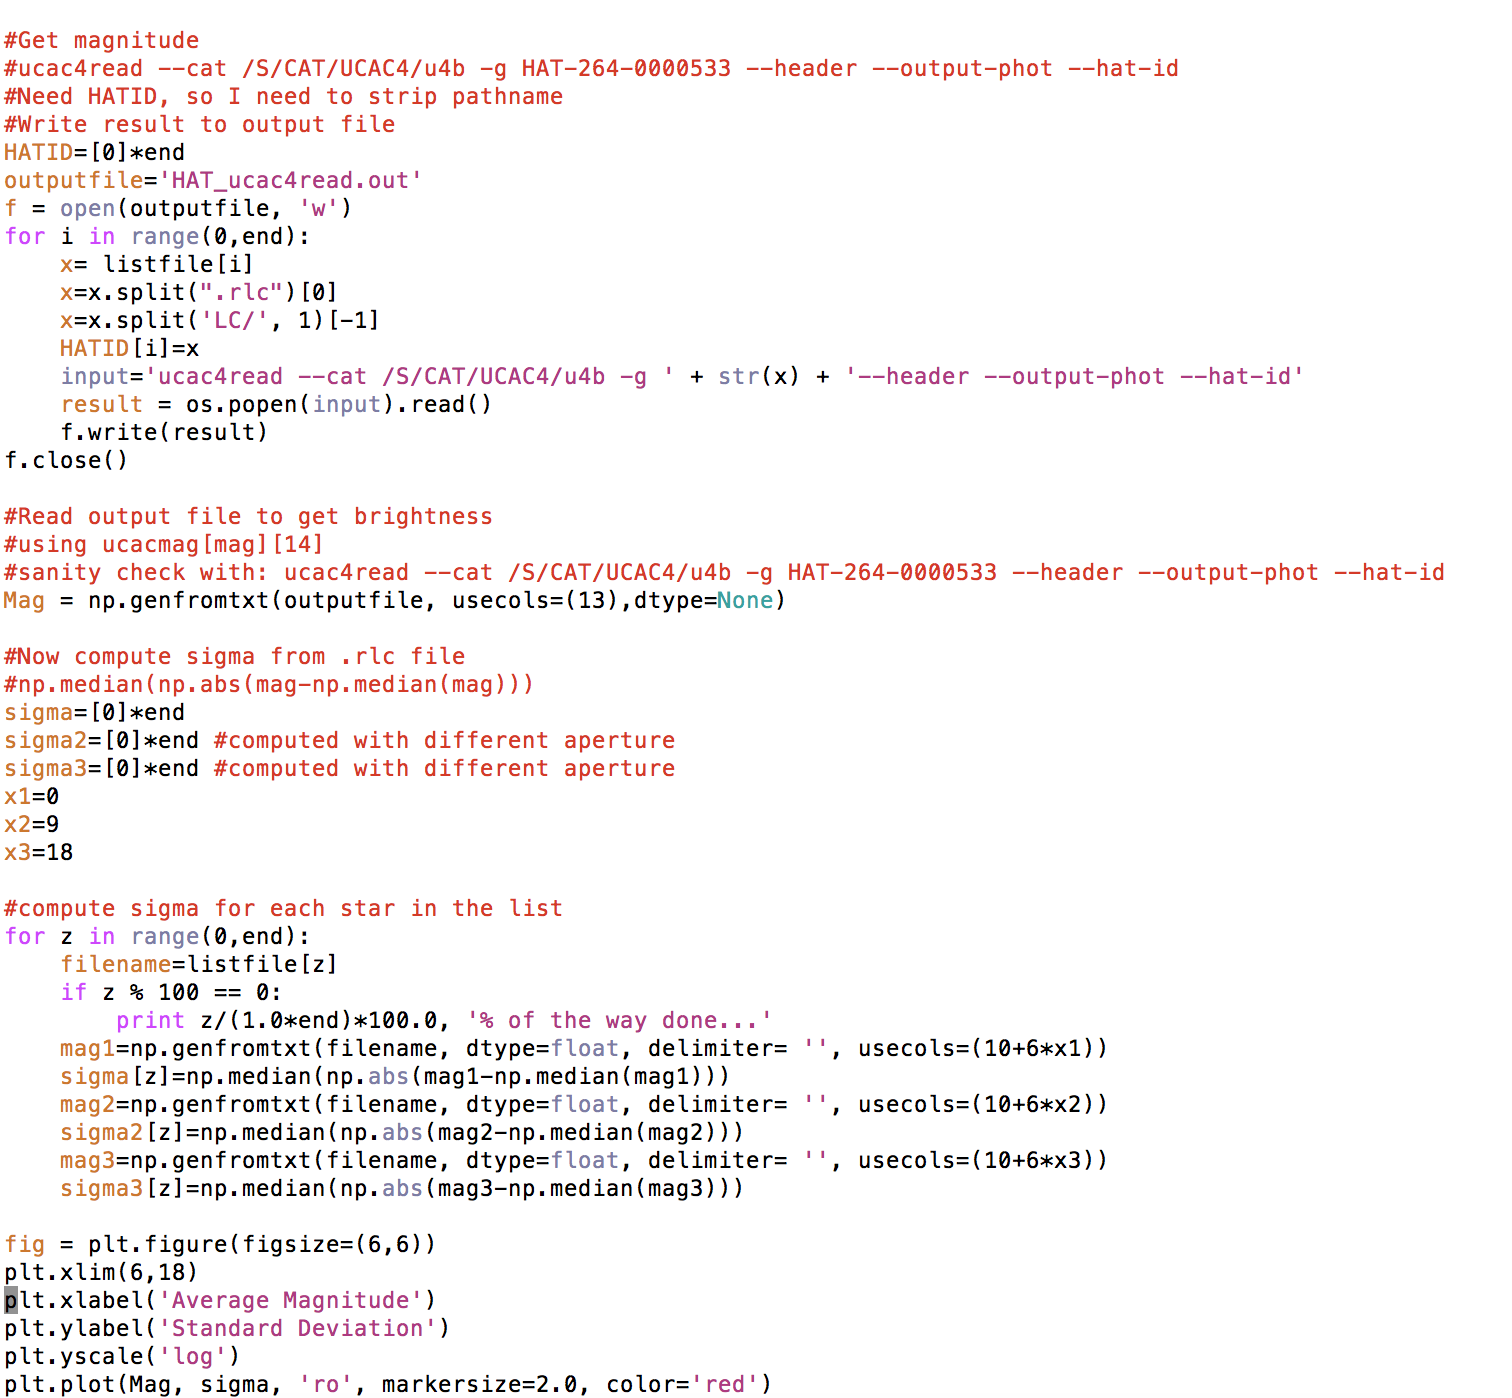
\includegraphics[width=\textwidth]{StndVMag.png}\\ 
\end{center}
To look up information on a particular star, use the \textbf{ucac4read} command, which will output the following information: HAT ID, RA, DEC, Object Type, whether or not it's a double star, magnitude, sigma of the mag, etc. 
The plots generated are shown below.
\begin{center}
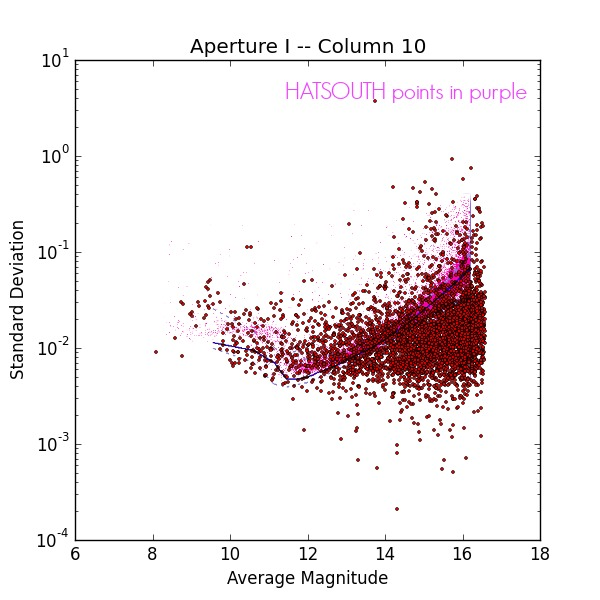
\includegraphics[width=0.8\textwidth]{Mag_Sigma1_comp.jpg}\\ 
\end{center}
\begin{center}
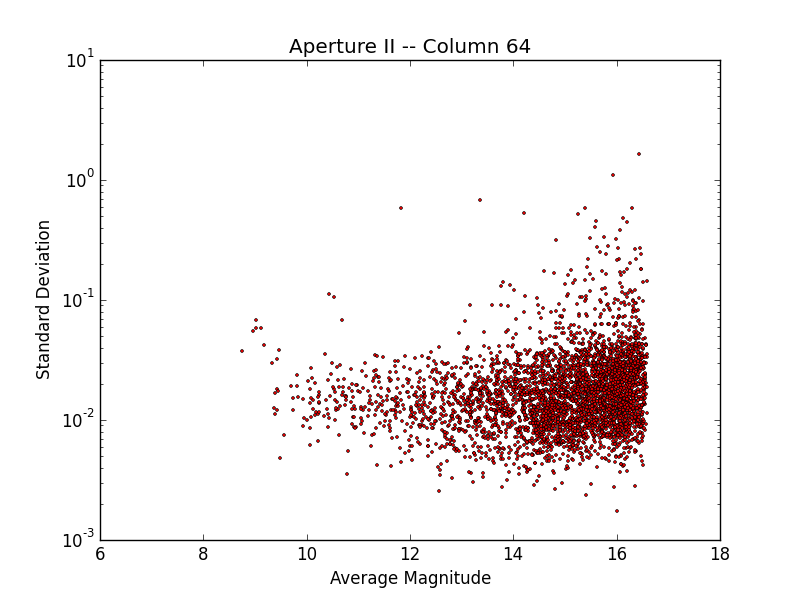
\includegraphics[width=0.8\textwidth]{Mag_Sigma2.png}\\ 
\end{center}
\begin{center}
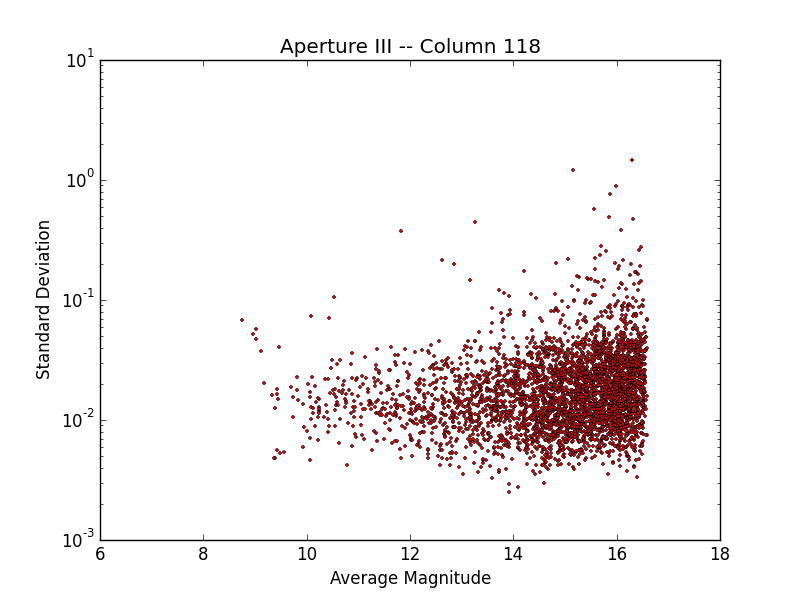
\includegraphics[width=0.8\textwidth]{Mag_Sigma3.png}\\ 
\end{center}
The three separate plots separated by a distinct aperture selection used to compute the standard deviation (np.median(np.abs(mag-np.median(mag))). Plots include all of the sources in the sub-frame. 
Unlike the example from the HATSouth survey, the overall structure is much more scattered about a more modestly increasing standard deviation for saturated stars. The standard deviation is lower for dimmer stars as compared to HATSOUTH, which you can see from the comparison plot (Mag\_Sigma1\_comp.jpg) where I have overplotted the HATSOUTH points you sent me as a reference. 
Chelsea says this difference in the scatter plots is due to blending. For many of the faint stars, we have counted lights leaking from neighboring bright stars, which make the photon noise smaller than it should be. 
\textcolor{purple}{\textit{Now I just need to do many group of experiments and have a set of these plots and pick the best. 
Chelsea says that the subtraction kernel setting is far from optimal. For raw light curves, we should be able to push down by an order of magnitude.}}

\pagebreak

\section*{Second Light Curve Batch Results: \hl{\textbf{b}/0, \textbf{i}/0, and \textbf{d}=1/1}}
\textbf{Changes made:} \\
I first made changes to the high resolution photometry with subtracted images. More specifically, I am adjust the tuning parameters: \textbf{b}, \textbf{i}, and \textbf{d}, which are set the script \textbf{melinda\_run\_ficonv.py}.
The first batch of light curves contained parameters: \textbf{b}/2, \textbf{i}/3, and \textbf{d}=3/3 \\
\textit{Remember \textbf{b} is the polynomial order fit to the background, so this was a second-order polynomial (likely too high), \textbf{i} was the order of the polynomial fit to the flux of the light curve, here a third-order polynomial (also likely too high), and \textbf{d=x/y} which is a ratio of the  half-size of the discrete kernel to the polynomial order \textbf{y} (again, probably too high).}\\
This second batch of light curves contains parameters: \textbf{b}/0, \textbf{i}/0, and \textbf{d}=1/1 \\
\textit{Files are simply overwritten and therefore I do not need to remove prior files.}\\
The \textbf{fiarith} command line subtraction is automated and already included in \textbf{melinda\_run\_ficonv.py}, so this process is completely streamlined. Next, I run the high-resolution photometry script \textbf{melinda\_run\_iphot.py}. This is followed by collecting the light curves with the bash script \textbf{melinda\_lc\_gen.sh}. This file takes a bit to run (also around 30 minutes or so). 
This will generate the light curves, which are located here: \textbf{/nfs/phs11/ar0/S/PROJ/msoares/201509\_K20\_ISM\_OpenClusters/IMSUB/LC}. \\
Again, I download all the data for this second batch.\\

\section*{Folding Light Curves}
I do not need to worry about folding light curves yet, as I still should focus on optimizing ims parameters. In the future, however, I will be folding candidate light curves.

\textcolor{purple}{\textbf{Next Mission: Generate Rotation Curve By End of November!}}\\ 
I do  not need to have the best precision to generate the rotation curve. The worst case will be just present the measurement for a few specific known targets. \textit{We might have enough time to reproduce the period .vs. B-V figure from the reference Chelsea sent me.} An example of such a plot from the Nardiello et al. 2014 paper is shown below. \\
\begin{center}
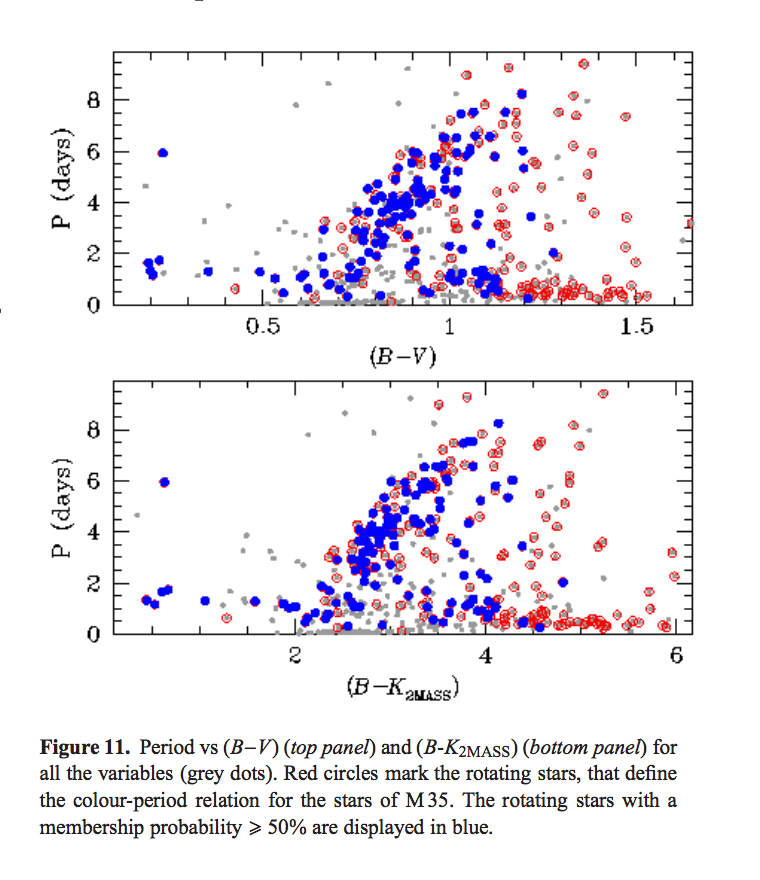
\includegraphics[width=0.4\textwidth]{reproduce2.png}
\end{center}

\section*{Organizing the Data}
\subsection*{GitHub: Bakos\_Project3}
On 10/27/2015 I created a Github repository to track the scripts in the subdirectory \textbf{/home/msoares/chelseasrc/ims}. This repository is currently public. \\
\textbf{IMPORTANT: if I want to permanently delete a file, don't only say \textbf{rm}, but use \textbf{git rm}, so that the repository will forget about it.}

\subsection*{Reorganizing Directories}
Chelsea has set up a directory called \textbf{/nfs/phs11/ar0/S/PROJ/hatuser/2015\_K2/experiments}.\\
Copy a version of the \textbf{setting.py} script I use in the experiment subdirectory to keep track of things. \\
Data files are now separated by photometry reference number. 
So far we have \textbf{ref\_2234} and \textbf{2334} only.
Chelsea is performing operations on the \textbf{2334} subdirectory, while I am adjusting the kernel parameters using a single photometry reference, \textbf{2234}. Files with adjusted parameters are organized into folders based on the selected kernel values. These include \textbf{b0i0d21}, \textbf{b0i0d22}, and \textbf{b1i1d21}.



\pagebreak
\section*{Papers to Read}

\subsection*{Recommended by J. Hartman}
\textit{Image Subtraction Using a Space-Varying kernel}\\
$ \hfill $ \url{http://aas.aanda.org/articles/aas/pdf/2000/11/ds8706.pdf}\\
\\
\textit{A METHOD FOR OPTIMAL IMAGE SUBTRACTION}\\
$ \hfill $ \url{http://iopscience.iop.org/article/10.1086/305984/pdf}\\
\\
\textit{FITSH -A Software Package for Image Processing}\\
$ \hfill $ \url{http://mnras.oxfordjournals.org/content/421/3/1825.full.pdf}\\

\subsection*{Recommended by Chelsea}
\textit{Selecting variable candidates in M35 and NGC 2158 from Asiago survey.}\\
$ \hfill $ \url{http://arxiv.org/pdf/1412.5688v1.pdf}\\ \\
$ \hfill $ \url{http://iopscience.iop.org/article/10.1088/0004-6256/150/1/10/pdf}\\ \\
$ \hfill $ \url{http://arxiv.org/pdf/1501.04416v1.pdf}

\pagebreak


\section*{Notes:}
Minor notes from  G\'{a}sp\'{a}r: consider doing image subtraction with double-sized reference frames. 

\pagebreak

\section*{11/02/2015}
Changes were made to \textbf{melinda\_run\_ficonv.py} to fix issues with the subtraction process. This is explained in the email below from Chelsea:\\
\begin{center}
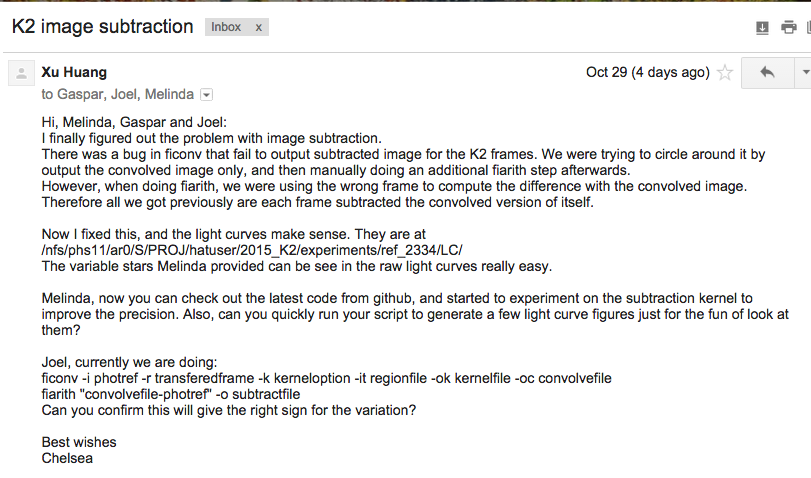
\includegraphics[width=\textwidth]{email1.png}\\
\end{center}
We still go with the -oc + fiarith until Chelsea fixes the bitpix problem.


\pagebreak

\title{Bakos_Project3}
{\Huge Switching Catalogs}\\[5mm]
After reviewing the Libralato, Bedin, Nardiello $\&$ Piotto (2015) paper (url listed below), Chelsea realized that one possible improvement we could make would be to update our catalog. We had been using a catalog named \textbf{photref.cat} which contained less than 10,000 sources. I took the variable sources listed in the Asiago Input Catalog, which contained more than 75,935 sources. Some of these sources were actually slightly outside the field of view of K2, so this was actually reduce to 66,486 sources in the end.  
I have placed the file \textbf{m35n2158\_kepmag.out} in the directory:\\ \textbf{/home/msoares/chelseasrc/ims/CATALOG}. 
Also in this subdirectory is the former catalog \textbf{photref.cat}. \\
The catalog contains the following information:
ID (integer number to identify source)   RA (J2000)   DEC (J2000)   Kepmag (mag)
Kepler magnitudes range from 7.5 to 31.2. 
The  catalog originally contained the sources in B-mag, V-mag, R-mag, J-mag, H-mag, K-mag, and instrument N-mag. More info on this catalog is given here. I had to convert these values to the Kepler magnitudes. To do this, I followed the logic given in the EPIC manual on page 10: \url{https://archive.stsci.edu/k2/epic.pdf}\\

Libralato et al. 2015 \url{http://arxiv.org/pdf/1510.09180v2.pdf}

\pagebreak
\title{Bakos_Project3}
{\Huge Kepler K2.2 -- Campaign 2 Project}\\[5mm]
On 12/15/2015 Chelsea suggested we consider exploring light curves in campaigns 2 and 5 as well. Campaign 2 has a superstamp for globular clusters M4 and M80, which enclose part of Upper Sco. Preparing one CCD is much faster than 84, so it really shouldn't take very long to explore this data set. 


\chapter*{Addressing Double catalog Entries}
There is a bug(/"feature") in the UCAC4 catalog in which certain sources that were resolved as multiple objects in some of the catalogs contributing to UCAC4, but only a single source in the 2MASS catalog, are given separate entries for each component in UCAC4. Each source has the same 2mass ID and is thus assigned the same HAT ID by our ucac4read code. The result is that I end up with a handful of sources having the same name in the cmrawphot file, leading to double entries for that id in the output photometry and double entries for each cadence in the light curve. \\ 
I see this problem for the following sources:
\begin{enumerate}
\item HAT-264-0576773
\item HAT-264-0011034
\item HAT-264-0003844
\item \sout{HAT-264-0345492} -- recently deleted because the file was null
\item \sout{HAT-264-0113691}
\item \sout{HAT-264-0001303}
\end{enumerate}

\textit{Did we keep these files?} -- yes, all files exist except those with the strike through in the list above. \\ \\
\textit{What do we do with these files?}\\
Joel says that it is not obvious what the best way to deal with this is. 
Obviously we need to fix something in the higher level catalog query step, but they haven't decided what that fix would be. 
We have previously discussed assigning new HATIDs to the fainter stars in each pair, but this requires fudging the 2MASS IDs in the catalog and we would still like to keep track of their original degenerate matches to 2MASS.  
Joel's suggestion would be to manually split the .rlc light curves into two for each of the objects above -- I can do this either by \textbf{relative position} or \textbf{reference brightness}.

I addressed this issue by writing a script in my ipython notebook that separated the .rlc files. The script is located at:
\begin{minted}{bash}
    /Users/msoares/Dropbox/K20/Notebooks/170504_SeparatingFiles.ipynb
\end{minted}

Only post-TFA .rlc files have been separated at this point. 

***To prevent this from happening in the future, I should add a step to the routine that generates the cmrawphot file to search for double entries and assign a new name to the second source (e.g., I might call it "HAT-264-0576773.2").


\chapter*{Investigating Reduced Light Curves to Find Candidates}
To perform the Box-fitting Least Squares (BLS) and the Lomb-Scargle algorithms (Scargle, 1982), I am using two methods: Joel Hartman's Vartools script and Waqas Bhatti's interactive, visually intuitive, and Astrobase code (written in Python). The Astrobase results are located right on my home computer with the final png files (containing post-TFA, pre-TFA, and Vartools pngs) located in the subdirectory below: 

\begin{minted}{bash}
     /Users/msoares/Dropbox/K20/Notebooks/LightCurve_PNG
\end{minted}

Those files, however, are not the primary sources used to cull with -- instead, we can refer to these files once interesting candidates have been selected through a more streamlined process.
We first find and classify interesting candidates interactively using Python pickles and Bhatti's Astrobase Checkplotserver webapp. This interface sets and saves variability tags, object type tags, best periods and epochs, and comments for each object using a browser-based UI. The information entered can then be exported as CSV or JSON for the next stage of work. An example of this process is shown here: \url{https://github.com/waqasbhatti/astrobase/blob/master/notebooks/lightcurves-and-checkplots.ipynb}

The pickle files are located at:
\begin{minted}{bash}
    /Users/msoares/Dropbox/K20/Notebooks/TFA_LC_PKL
\end{minted}

We make a \texttt{.json} file using the command:
\begin{minted}{bash}
	checkplotlist pkl .
\end{minted}
Now you want to view them on with checkplotserver...make sure you are using Python version 3 first!
You then simply open the interactive, checkplotserver app by typing:
\begin{minted}{bash}
	checkplotserver
\end{minted}
The interactive webpage will look something like this.
\begin{center}
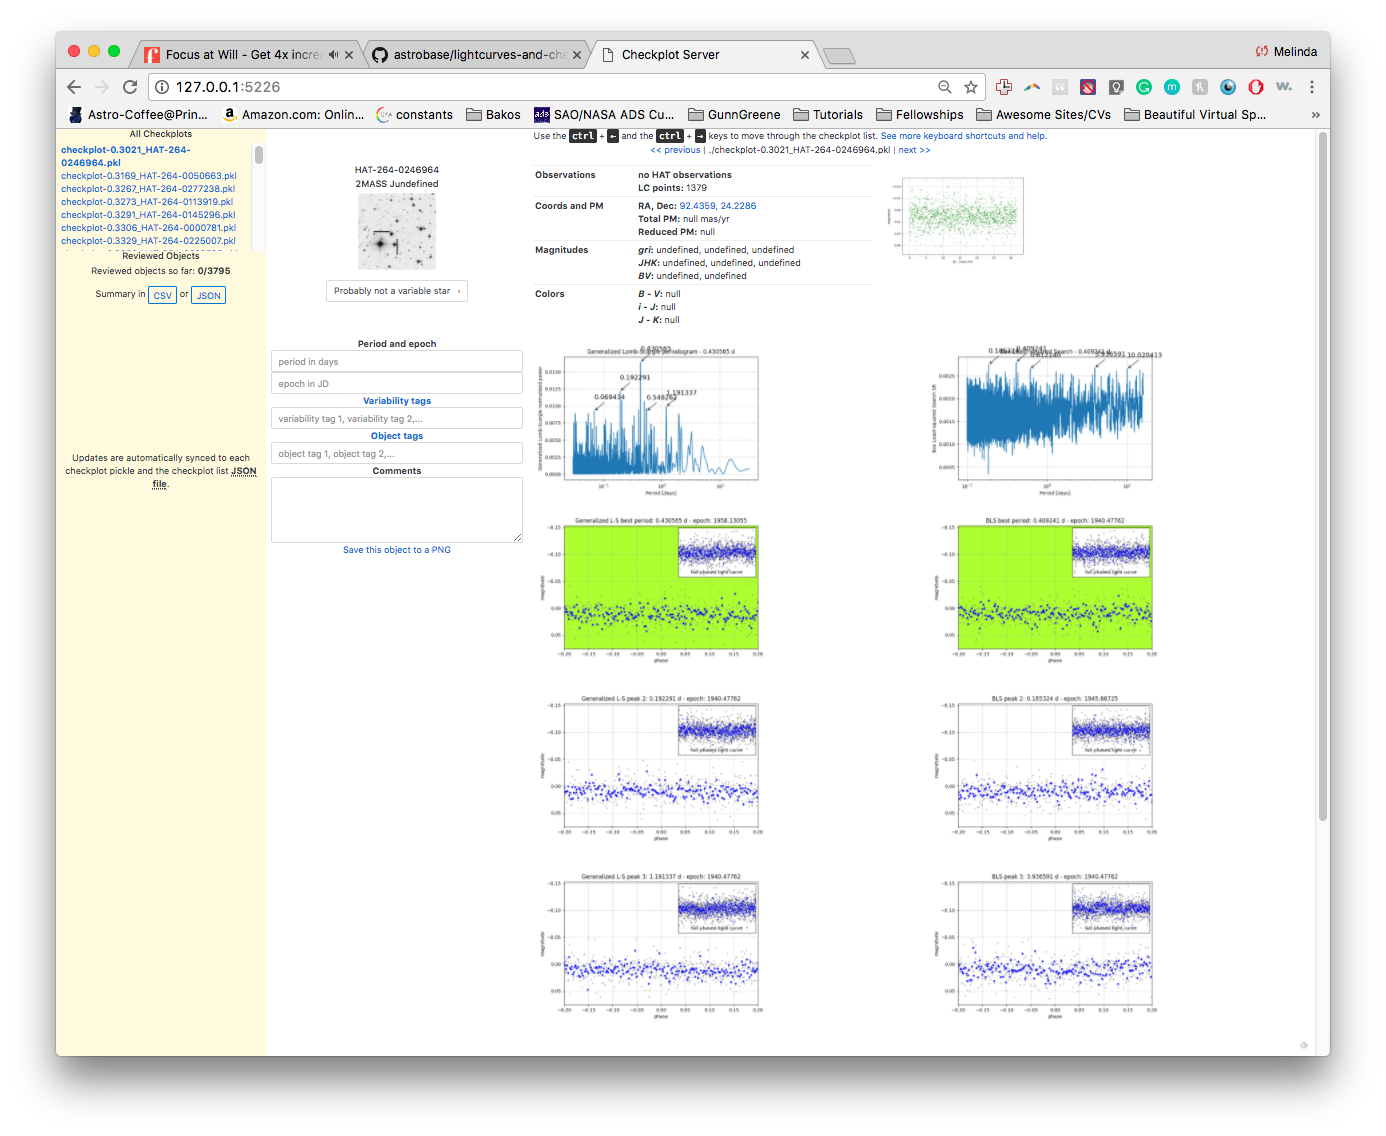
\includegraphics[width=0.7\textwidth]{checkplotserver.png}\\
\end{center}
When you save objects as a .png file, they will save within the same \texttt{TFA\_LC\_PKL} subdirectory, so you'll need to move them to an appropriate folder. 


\subsection*{Vartools Output Lightcurves}
The Vartools output files, on the other hand, are located on the phs11 machine at the subdirectory:

\begin{minted}{bash}
     /home/msoares/chelseasrc/ims/BLS/BLS_1
\end{minted}
Here there are two types of files, the phase curve, which contains phase information and the magnitude of the model, ends in *.rlc.tfalc.bls.phcurve, while those ending in *.rlc.tfalc.bls.model contain the model. The plot shown in Figure~\ref{finalfile} only relies on the contents of the *.rlc.tfalc.bls.phcurve files. 

\chapter*{Running Parallelized Scripts for Faster Analysis}
\section*{Using ipyparallel}
I got another technically helpful email from Waqas explaining how to use ipyparallel to run BLS and LS algorithms using his Astrobase software. You cannot just use multiprocessing.Pool here, as it will error out due to the spawning of daemonic processes. 
I can still run stuff in parallel, but only if I switch
to ipyparallel as the driver instead of multiprocessing.Pool. This
mostly follows the advice in the notebook:
\url{https://github.com/waqasbhatti/astrobase/blob/master/notebooks/parallel-ipython.ipynb}

Essentially, I run ipyparallel workers on the same machine instead of across a cluster. How do I do this?

With your virtualenv activated:
\begin{minted}{bash}
    (venv)$ pip install ipyparallel
\end{minted}
That will install the driver and workers.

Then to start a cluster on phs11 with 4 workers (as laid out before):
\begin{minted}{bash}
    (venv)$ ipcluster start -n 4 &
\end{minted}

Then I simply follow the notebook from ``set up the cluster view" onwards.
The function I map across the whole cluster is my
worker function that I set up for use with multiprocessing.Pool. The function call is very similar:

\begin{minted}{bash}
    results = dview.map_sync(do_lc_stuff, lclist)
\end{minted}

A final version of this working script is available at 
\begin{minted}{bash}
    /home/msoares/chelseasrc/ims/Astrobase/Parallel_MakeTFA_LC_PNG_Vartools.py
\end{minted}

\section*{Submit with nohup}
Pipes break and they break often, as a result, you really need to use nohup with all file submissions. Here is an example of how to run your parallelized script using nohup to prevent these issues.

\begin{minted}{bash}
    (venv)$ nohup ipcluster -n 4 >> error-log.txt &

    (venv)$ nohup python /path/to/your/script.py >> error-log.txt &
\end{minted}


%%%%%CAMPAIGN 5 -- IGNORE FOR NOW%%%%%%%%%%%%%%%%%%%%%%%%%
\chapter*{Campaign 5}
{\Huge Kepler K2.5 -- Campaign 5 Project}\\[5mm]
On 12/15/2015 Chelsea suggested we consider exploring light curves in campaigns 2 and 5 as well. There is an M67 superstamp which includes the Beehive. 
Preparing one CCD is much faster than 84, so it really shouldn't take very long to explore this data set. 

\end{document}